\newcommand{\rnd}[2]{\mathrm{rnd}(#1,#2)}


\subsection{The PBM Model}

\subsubsection{Introduction}
In order to be able to investigate the influence of money and social inequalities, we derived a model from the model proposed by XXXX. We name this model the PBM model, to underline the high importance that Productivity, Boredom and Money play in the model.

\subsubsection{Basic principle}
The PBM model describes the dynamics of the work allocation of different taks in a society of workers. 
A worker is not equally skilled for all of the tasks; we define his \emph{productivity} for a task as the amount of work (or produced units) in a given time. 
The productivity of a worker for a given tasks evolves with time, depending on whether he is actually performing the task or not, which reproduces learning and forgetting. Similarly, the \emph{boredom} of the worker regarding the tasks evolves. For a worker, the boredom is equivalent to earning less money.
Each worker is remunerated for his work; as all the tasks are considered to be equally important for the society, they all deliver the same total amount of money, which is distributed to the workers proportionally to their productivity.
Every now and then, the worker is given the possibility to quit his task and choose another task, which he will do if he can get a better salary/boredom balance. 


\subsubsection{Explanation of the model}
The initial value for the productivity $P_{ij}$ of worker $i$ at task $j$ is generated randomly according to the equation
\begin{equation}
	P_{ij}(t_0) = \rnd{P_\mu}{P_\sigma}
\end{equation}
where $\rnd{\mu}{\sigma}$ means that the number is generated according to a normal distribution of mean $\mu$ and standard deviation $\sigma$.

As a first task, a worker will choose the task where his productivity is highest.

In order to describe the fact that some people intrinsically learn faster than other people and have more room for improvement, each worker $i$ is attributed a task-independent \emph{ability} $A_i$, which is time-independent and generated randomly according to
\begin{equation}
	A_{i} = \rnd{A_\mu}{A_\sigma}
\end{equation}
The maximal productivity of worker $i$ at task $j$ is directly related to his initial productivity at this task and his ability:
\begin{equation}
	P_{ij}^\textrm{max} = A_i \cdot P_{ij}(t_0)
\end{equation}
The productivity evolves in time as a function of the learning factor $\lambda$ and of the forgetting factor $\kappa$, 
\begin{equation}
	P_{ij}(t+\Delta t) = \begin{cases}
		P_{ij}(t) + (P_{ij}^\textrm{max}-P_{ij}(t)) \cdot \lambda \Delta t & \text{if worker $i$ is performing task $j$}\\
		P_{ij}(t) - P_{ij}(t) \cdot \kappa \Delta t & \text{otherwise}\\
		\end{cases}
\end{equation}
where $\Delta t$ is the time step for the time evolution.

The boredom $B_{ij}$ of worker $i$ at task $j$ is initially zero at time $t_0$. The maximal boredom $B_{ij}^\textrm{max}$ is generated randomly by the following formula:
\begin{equation}
	B_{ij}^\textrm{max} = \rnd{B_\mu}{B_\sigma}
\end{equation}
The evolution of the boredom evolves in a similar fashion as the productivity and depends on the parameters $\zeta$ and $\eta$ for the boredom increase and decrease, respectively:
\begin{equation}
	B_{ij}(t+\Delta t) = \begin{cases}
		B_{ij}(t) + (B_{ij}^\textrm{max}-B_{ij}(t)) \cdot \zeta \Delta t & \text{if worker $i$ is performing task $j$}\\
		B_{ij}(t) - B_{ij}(t) \cdot \eta \Delta t & \text{otherwise}\\
		\end{cases}
\end{equation}
For a worker, boredom is equivalent to earning less money than granted by his productivity. The ``felt'' salary is given by the result of the substraction of the boredom $B_{ij}(t)$ at the current task from the earned money.

The \emph{job offer frequency} $p_s$ is responsible for the occasional possibility given to the worker to change his task: at each time step, a worker has this choice if a random number distributed uniformly between $0$ and $1$ is smaller than $p_s$.

\subsubsection{Results and Discussion}
The MMM model is quite robust and the variation of the parameters allows several findings. 
Parameters for a standard simulation could be the following: $N=7$, $M=3$, $\lambda=0.01$, $\kappa=0.003$, $\zeta=0.001$, $\eta=0.0003$, $p_s=0.003$, $\Delta t=1$, $A_\mu=3$, $A_\sigma=0.7$, $P_\mu=2$, $P_\sigma=0.7$, $B_\mu=0.5$, $B_\sigma=0.15$. Figure~\ref{fig:sim1task} shows the time evolution of the tasks performed by the different workers. It allows to see the dynamics of work allocation. Figures~\ref{fig:sim1prod}, \ref{fig:sim1money} and \ref{fig:sim1boredom} allow to understand the motivation for choosing another task. Figure~\ref{fig:sim1prod} shows the evolution of the productivity at the current tasks and explains why workers performing the same task do not earn the same amount of money, which can be seen in Figure~\ref{fig:sim1money}. Figure~\ref{fig:sim1boredom} displays the evolution of the boredom. It illustrates that a too high boredom can induce a change of task even if the new task is less paid than the previous one. A general observation is that people working on tasks at which their maximam boredom is high tend to change the task rapidly because of the rapid increase of the boredom. Figure~\ref{fig:sim1totalmoney} shows the total amount of money earned so far by each of the workers. It features a pronounced social inequality, which is caused by two main factors. Firstly, the inherent characteristics of the workers make some of them much more productive, thence earning more money. The second factor is has its origin in the society, more precisely in the production of other individuals; it could be illustrated by the fact that a not particularly skilled individual will be remunerated a lot if he is the only one able to do his job, while two very skilled individuals at the same task will earn much less.

\begin{figure}[h!]
	\centering
	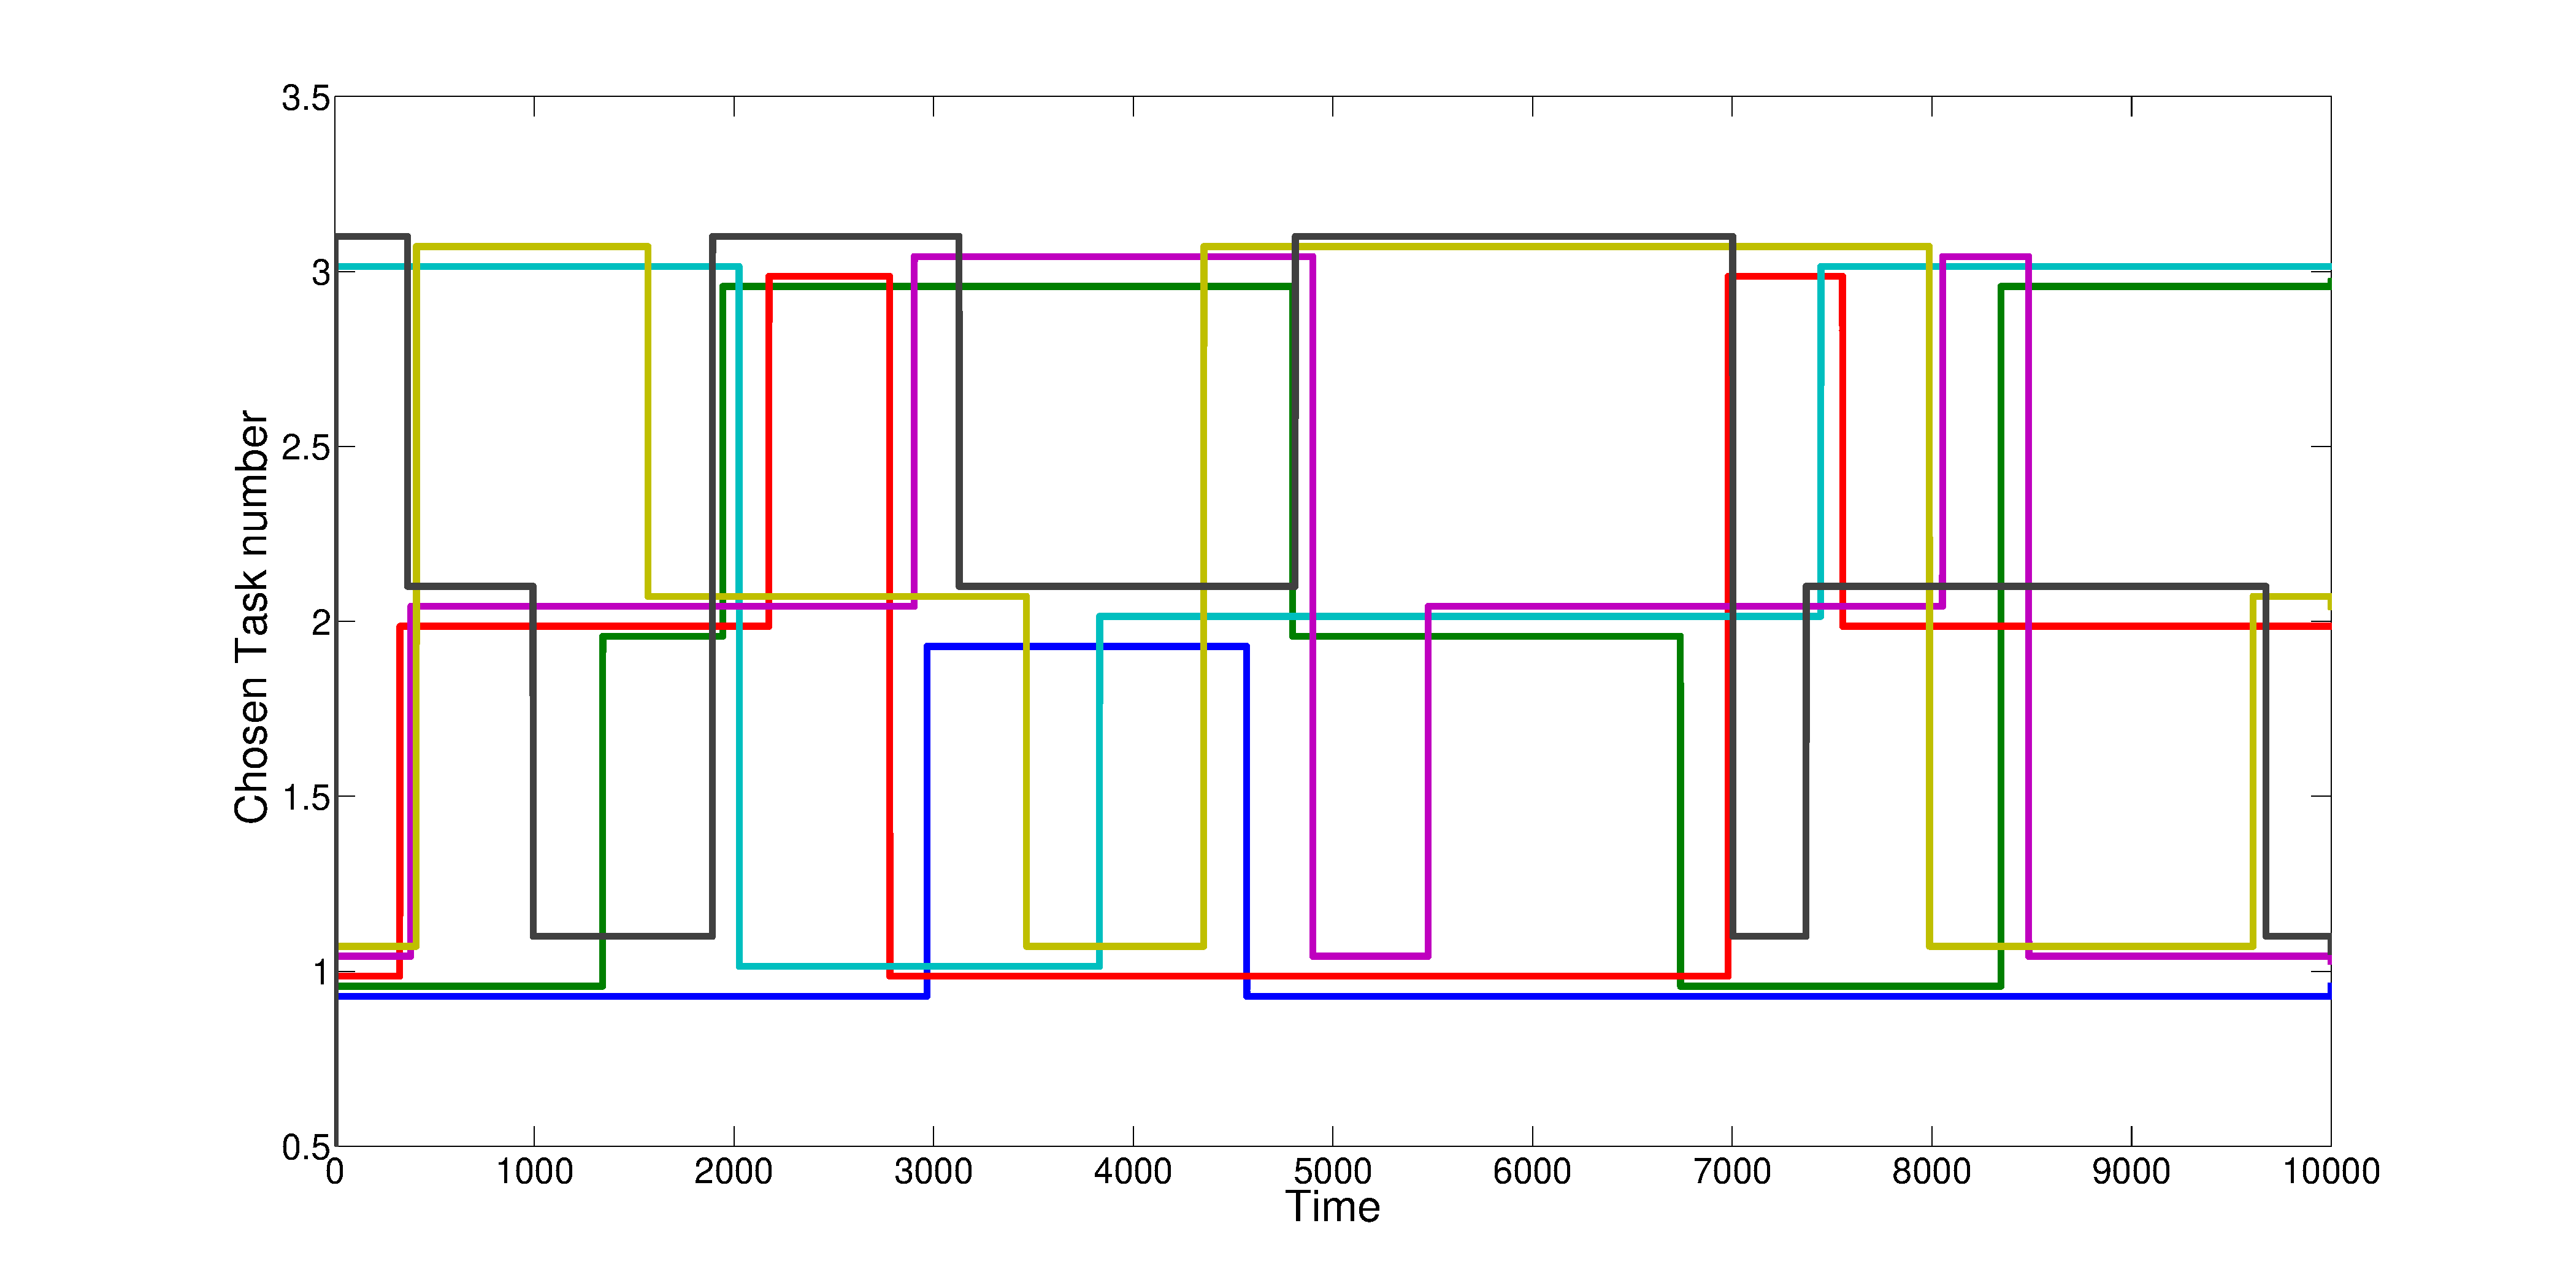
\includegraphics[width=0.9\textwidth]{../figures/taskno.pdf}
	\caption{Current tasks of the workers as a function of time. Each worker is represented by a different color. The curves of the different individui have a small vertical shift so that all the lines are visible.}
	\label{fig:sim1task}
\end{figure}

\begin{figure}[h!]
	\centering
	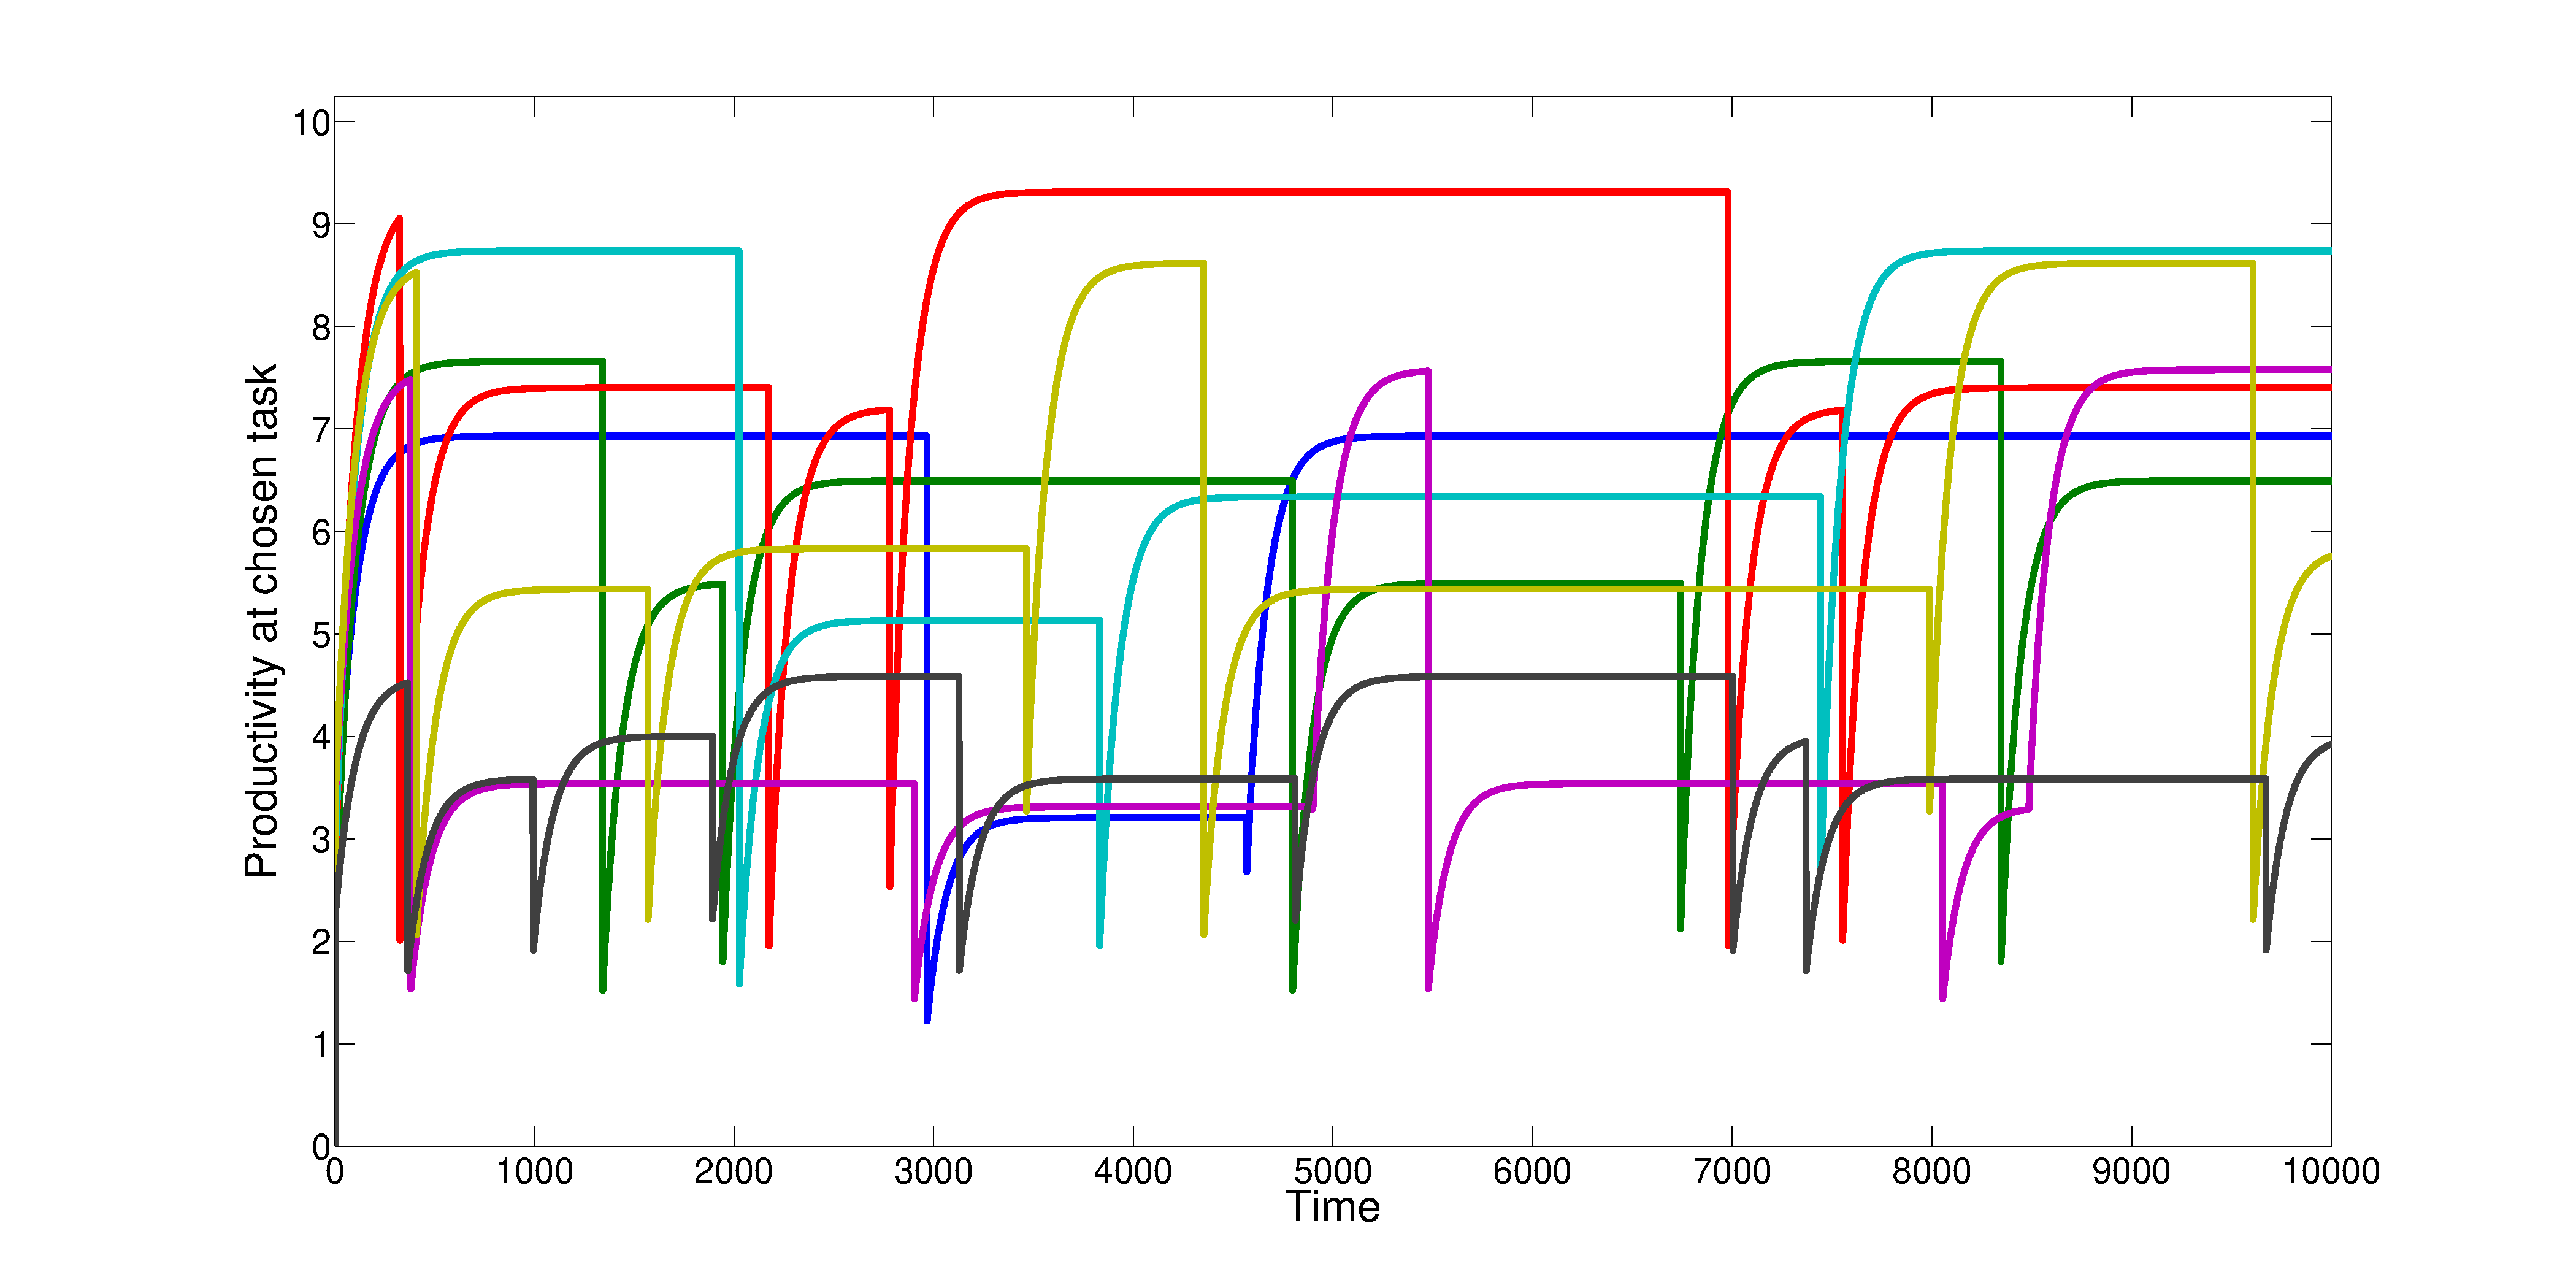
\includegraphics[width=0.9\textwidth]{../figures/productivity.pdf}
	\caption{Productivity of the workers at the tasks they are currently performing. The incontinuities mark a change in the task and correspond to what is shown in Figure~\ref{fig:sim1task}.}
	\label{fig:sim1prod}
\end{figure}

\begin{figure}[h!]
	\centering
	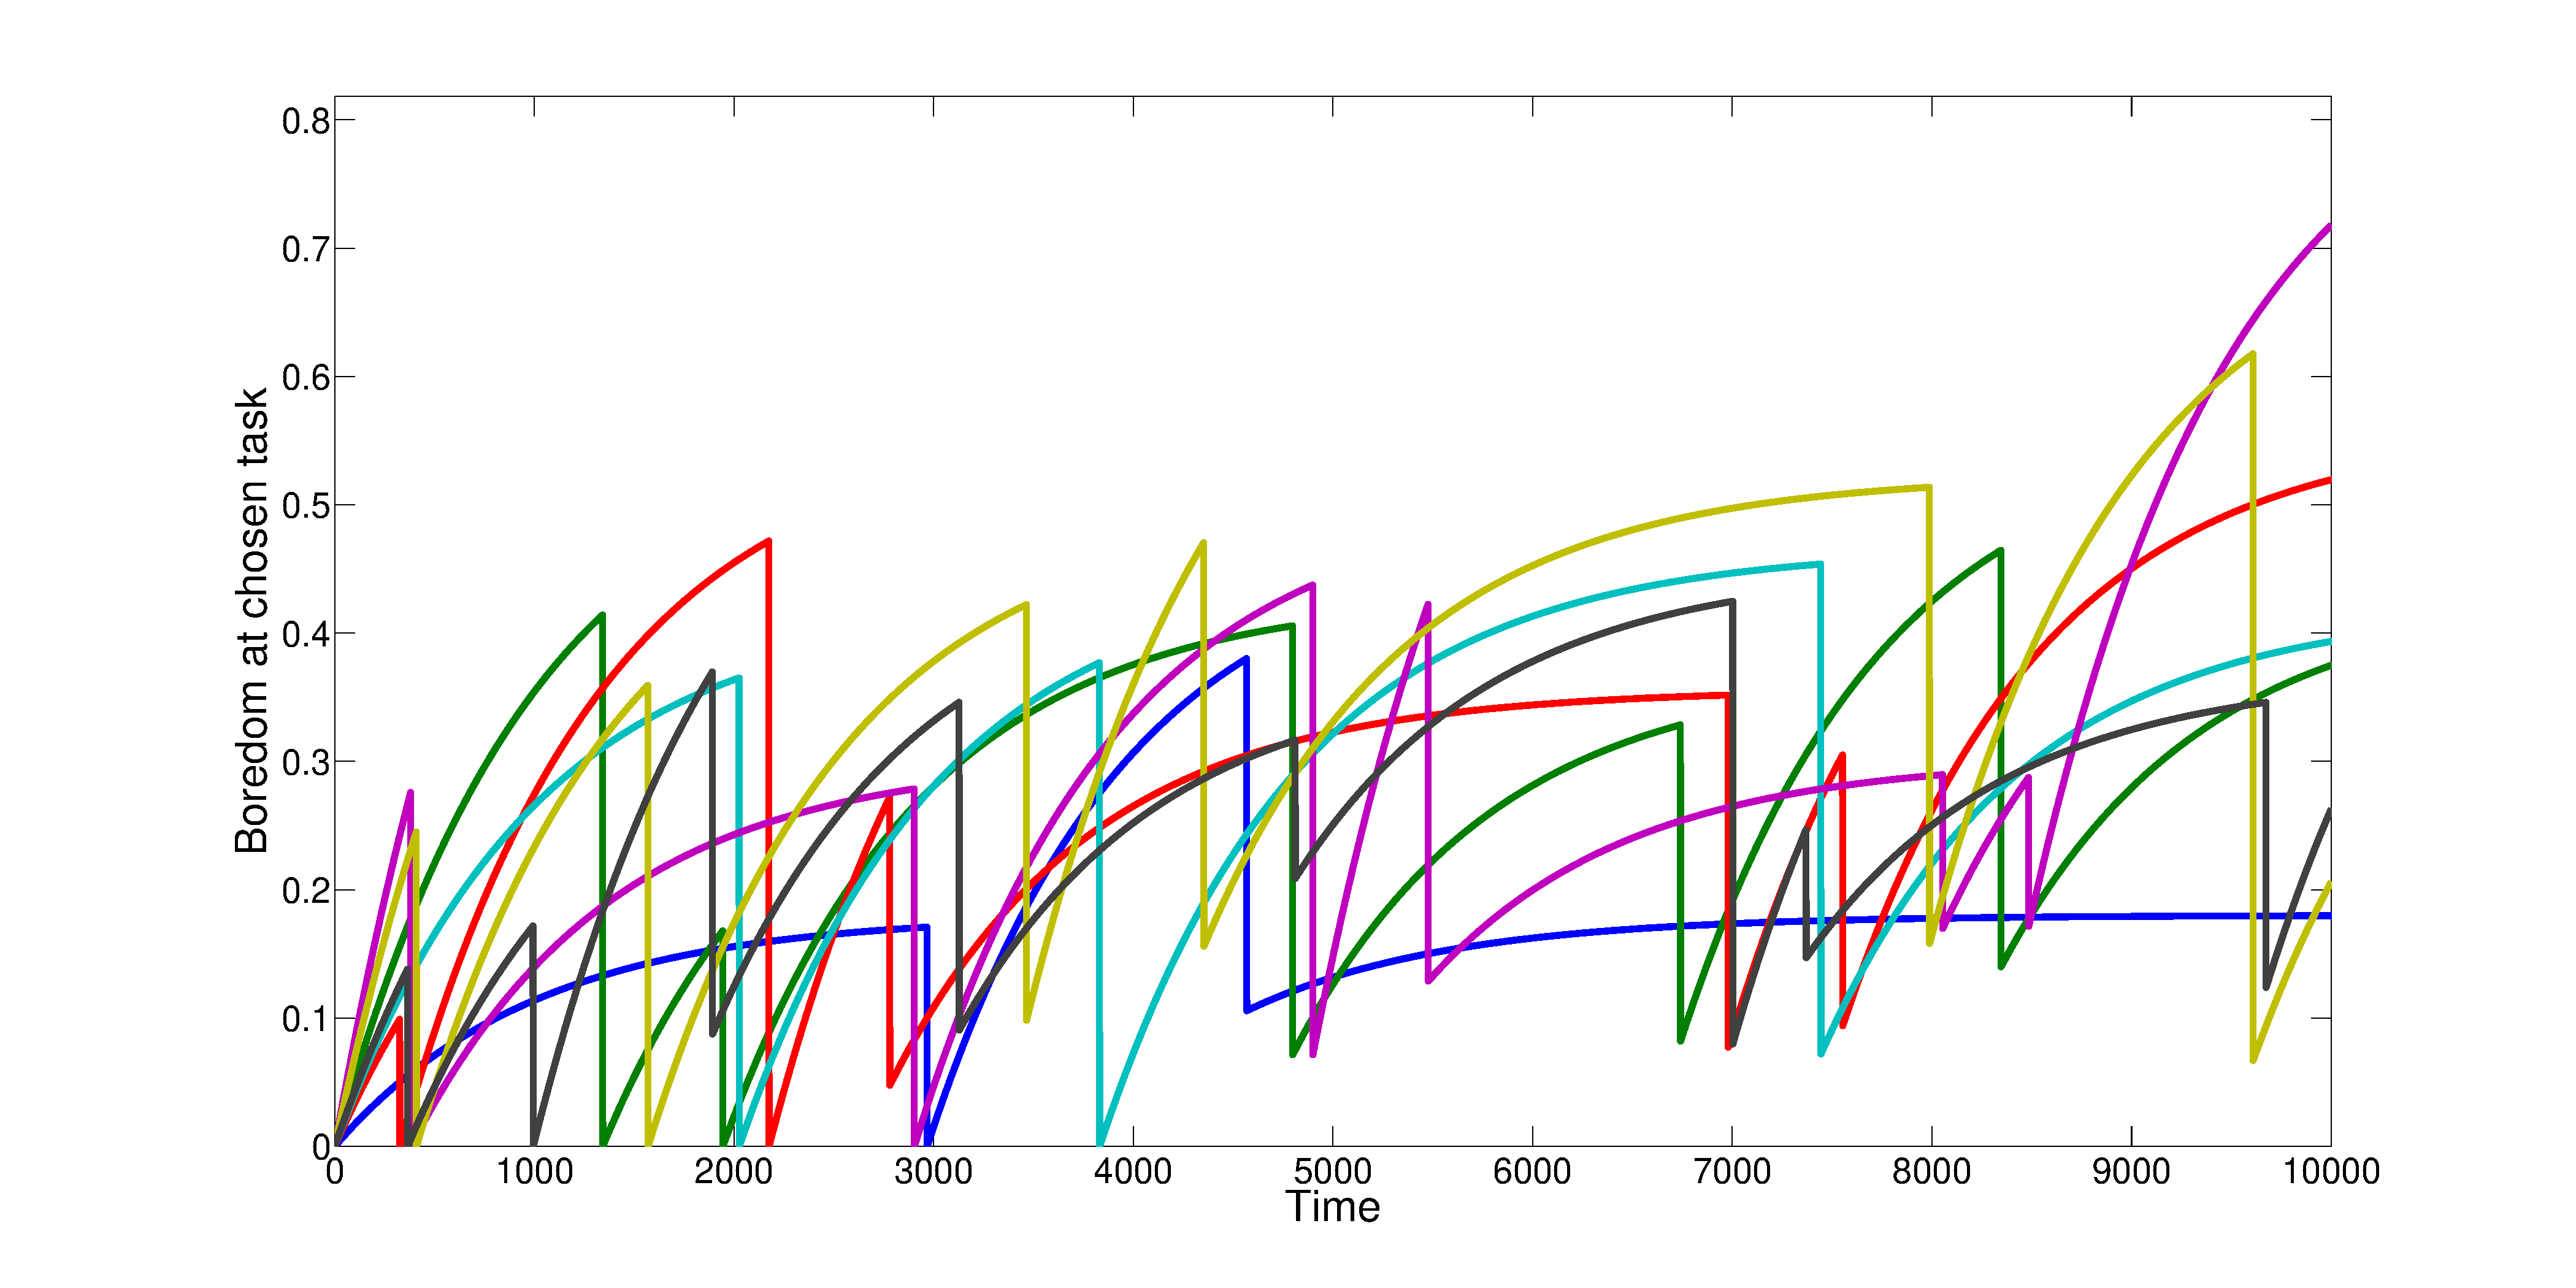
\includegraphics[width=0.9\textwidth]{../figures/boredom.pdf}
	\caption{Boredom of the workers at the tasks they are currently performing. It can be seen that the maximal boredom is not achieved in most of the cases, since the boredom becomes too high.}
	\label{fig:sim1boredom}
\end{figure}

\begin{figure}[h!]
	\centering
	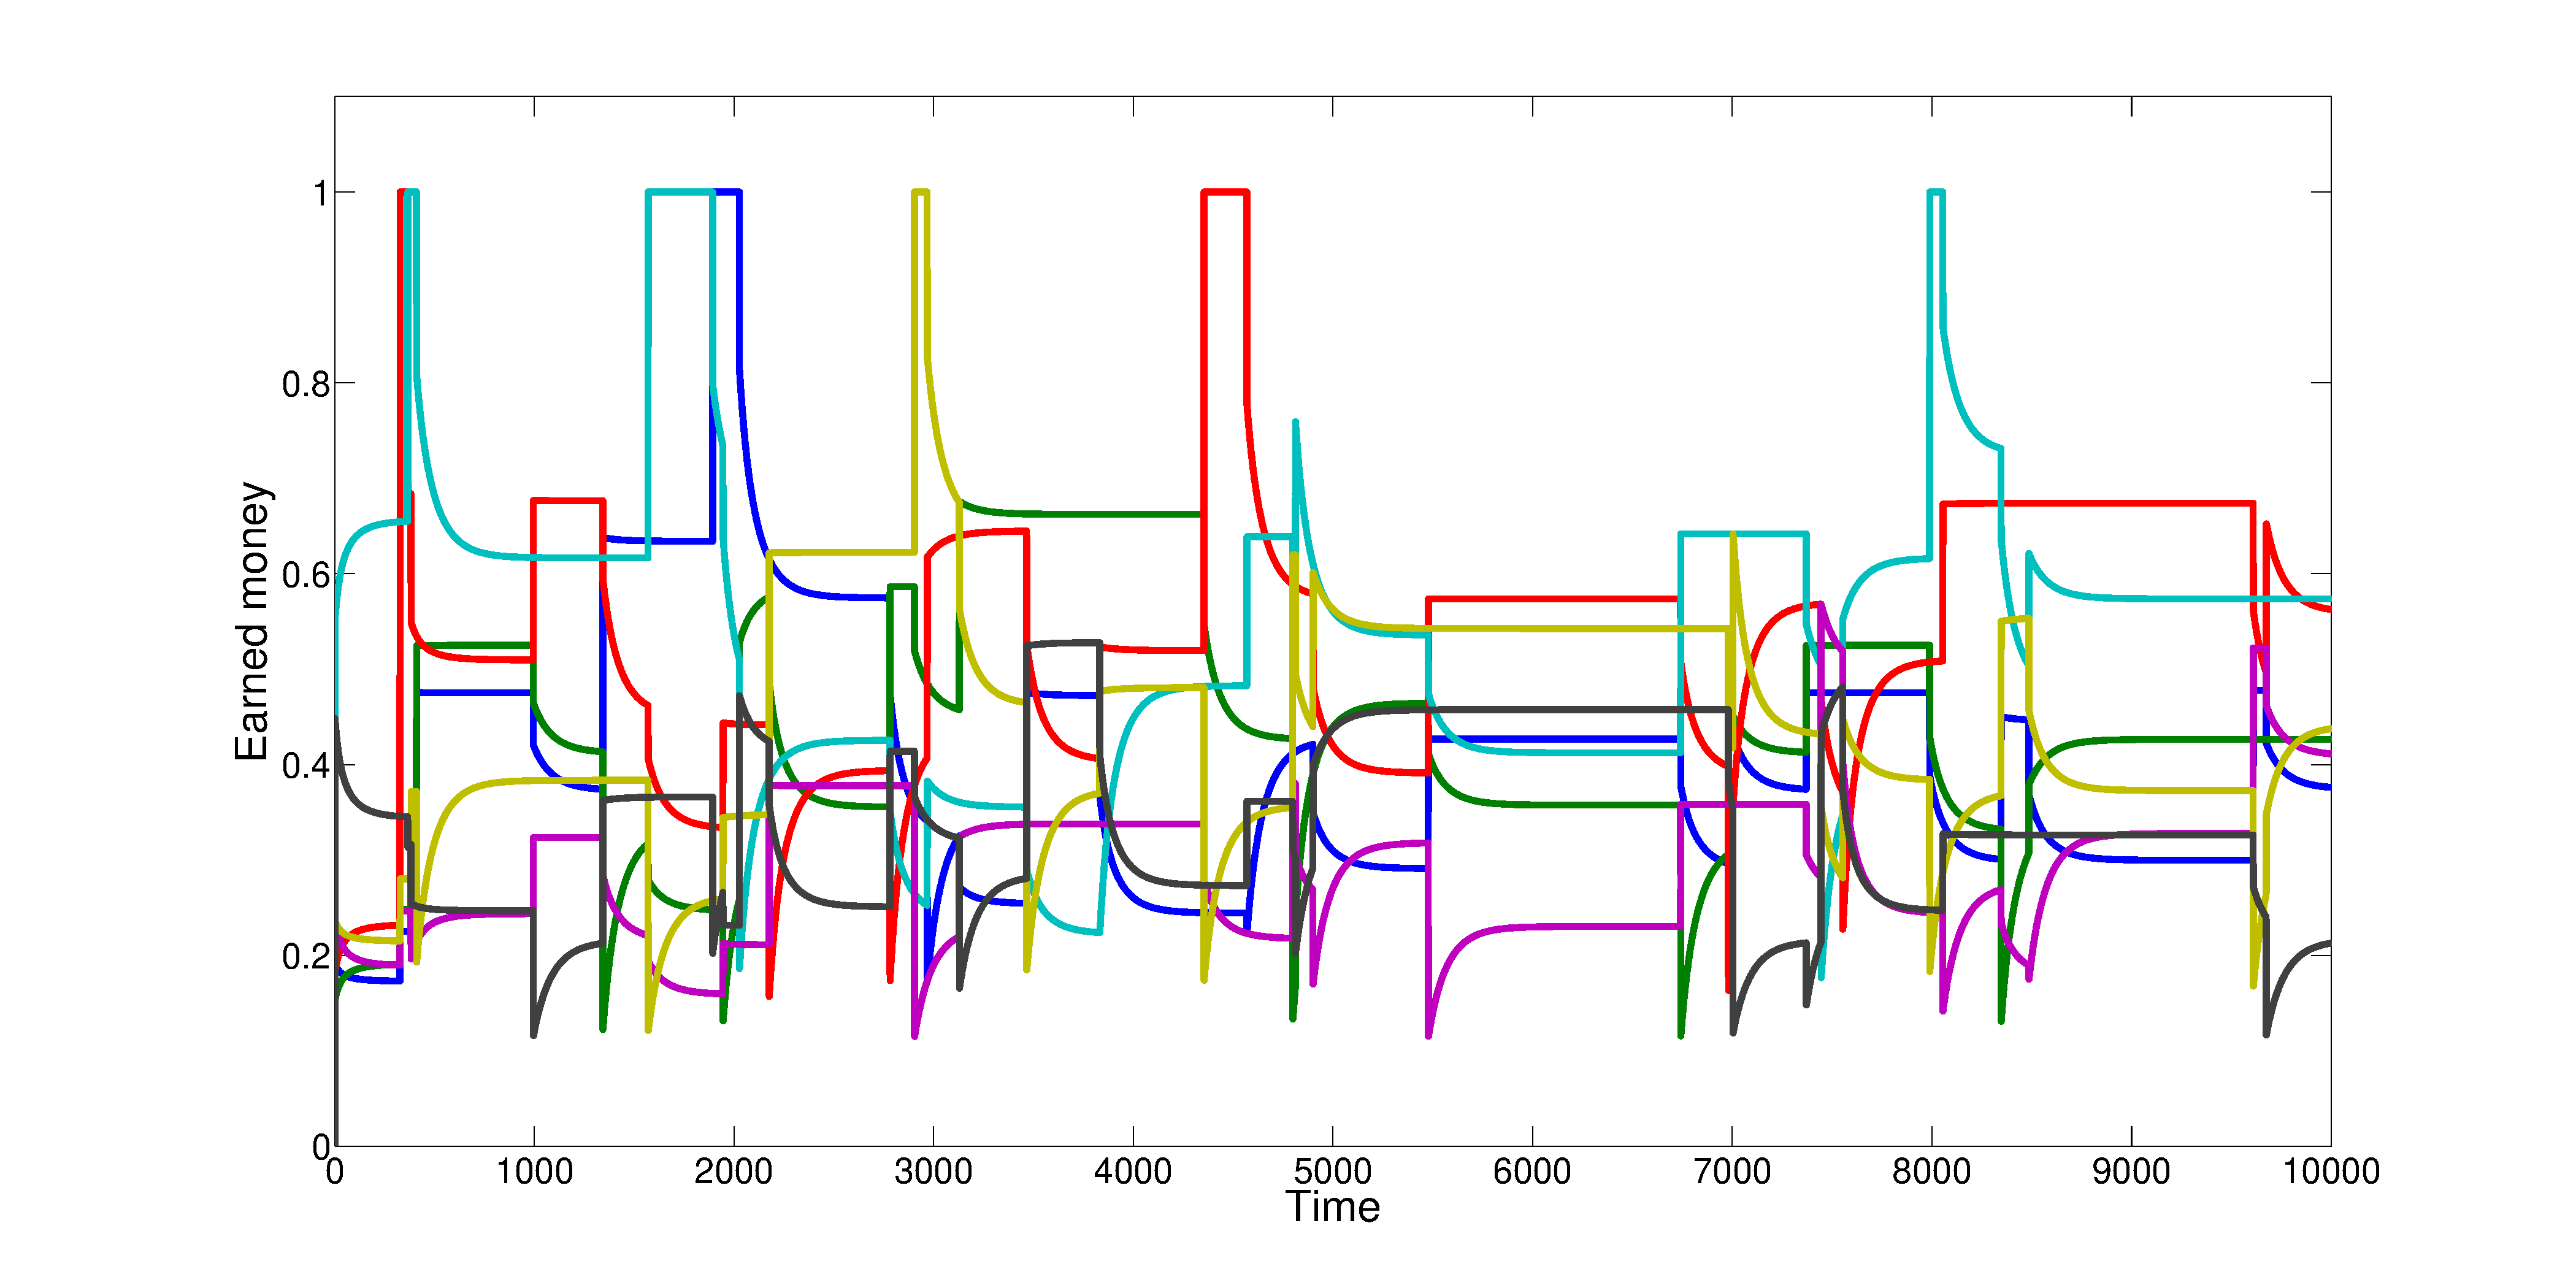
\includegraphics[width=0.9\textwidth]{../figures/money.pdf}
	\caption{Salary of the workers as a function of time. A salary of 1 means that a worker is the only one to perform his current task and therefore gets all the money granted to the task.}
	\label{fig:sim1money}
\end{figure}

\begin{figure}[h!]
	\centering
	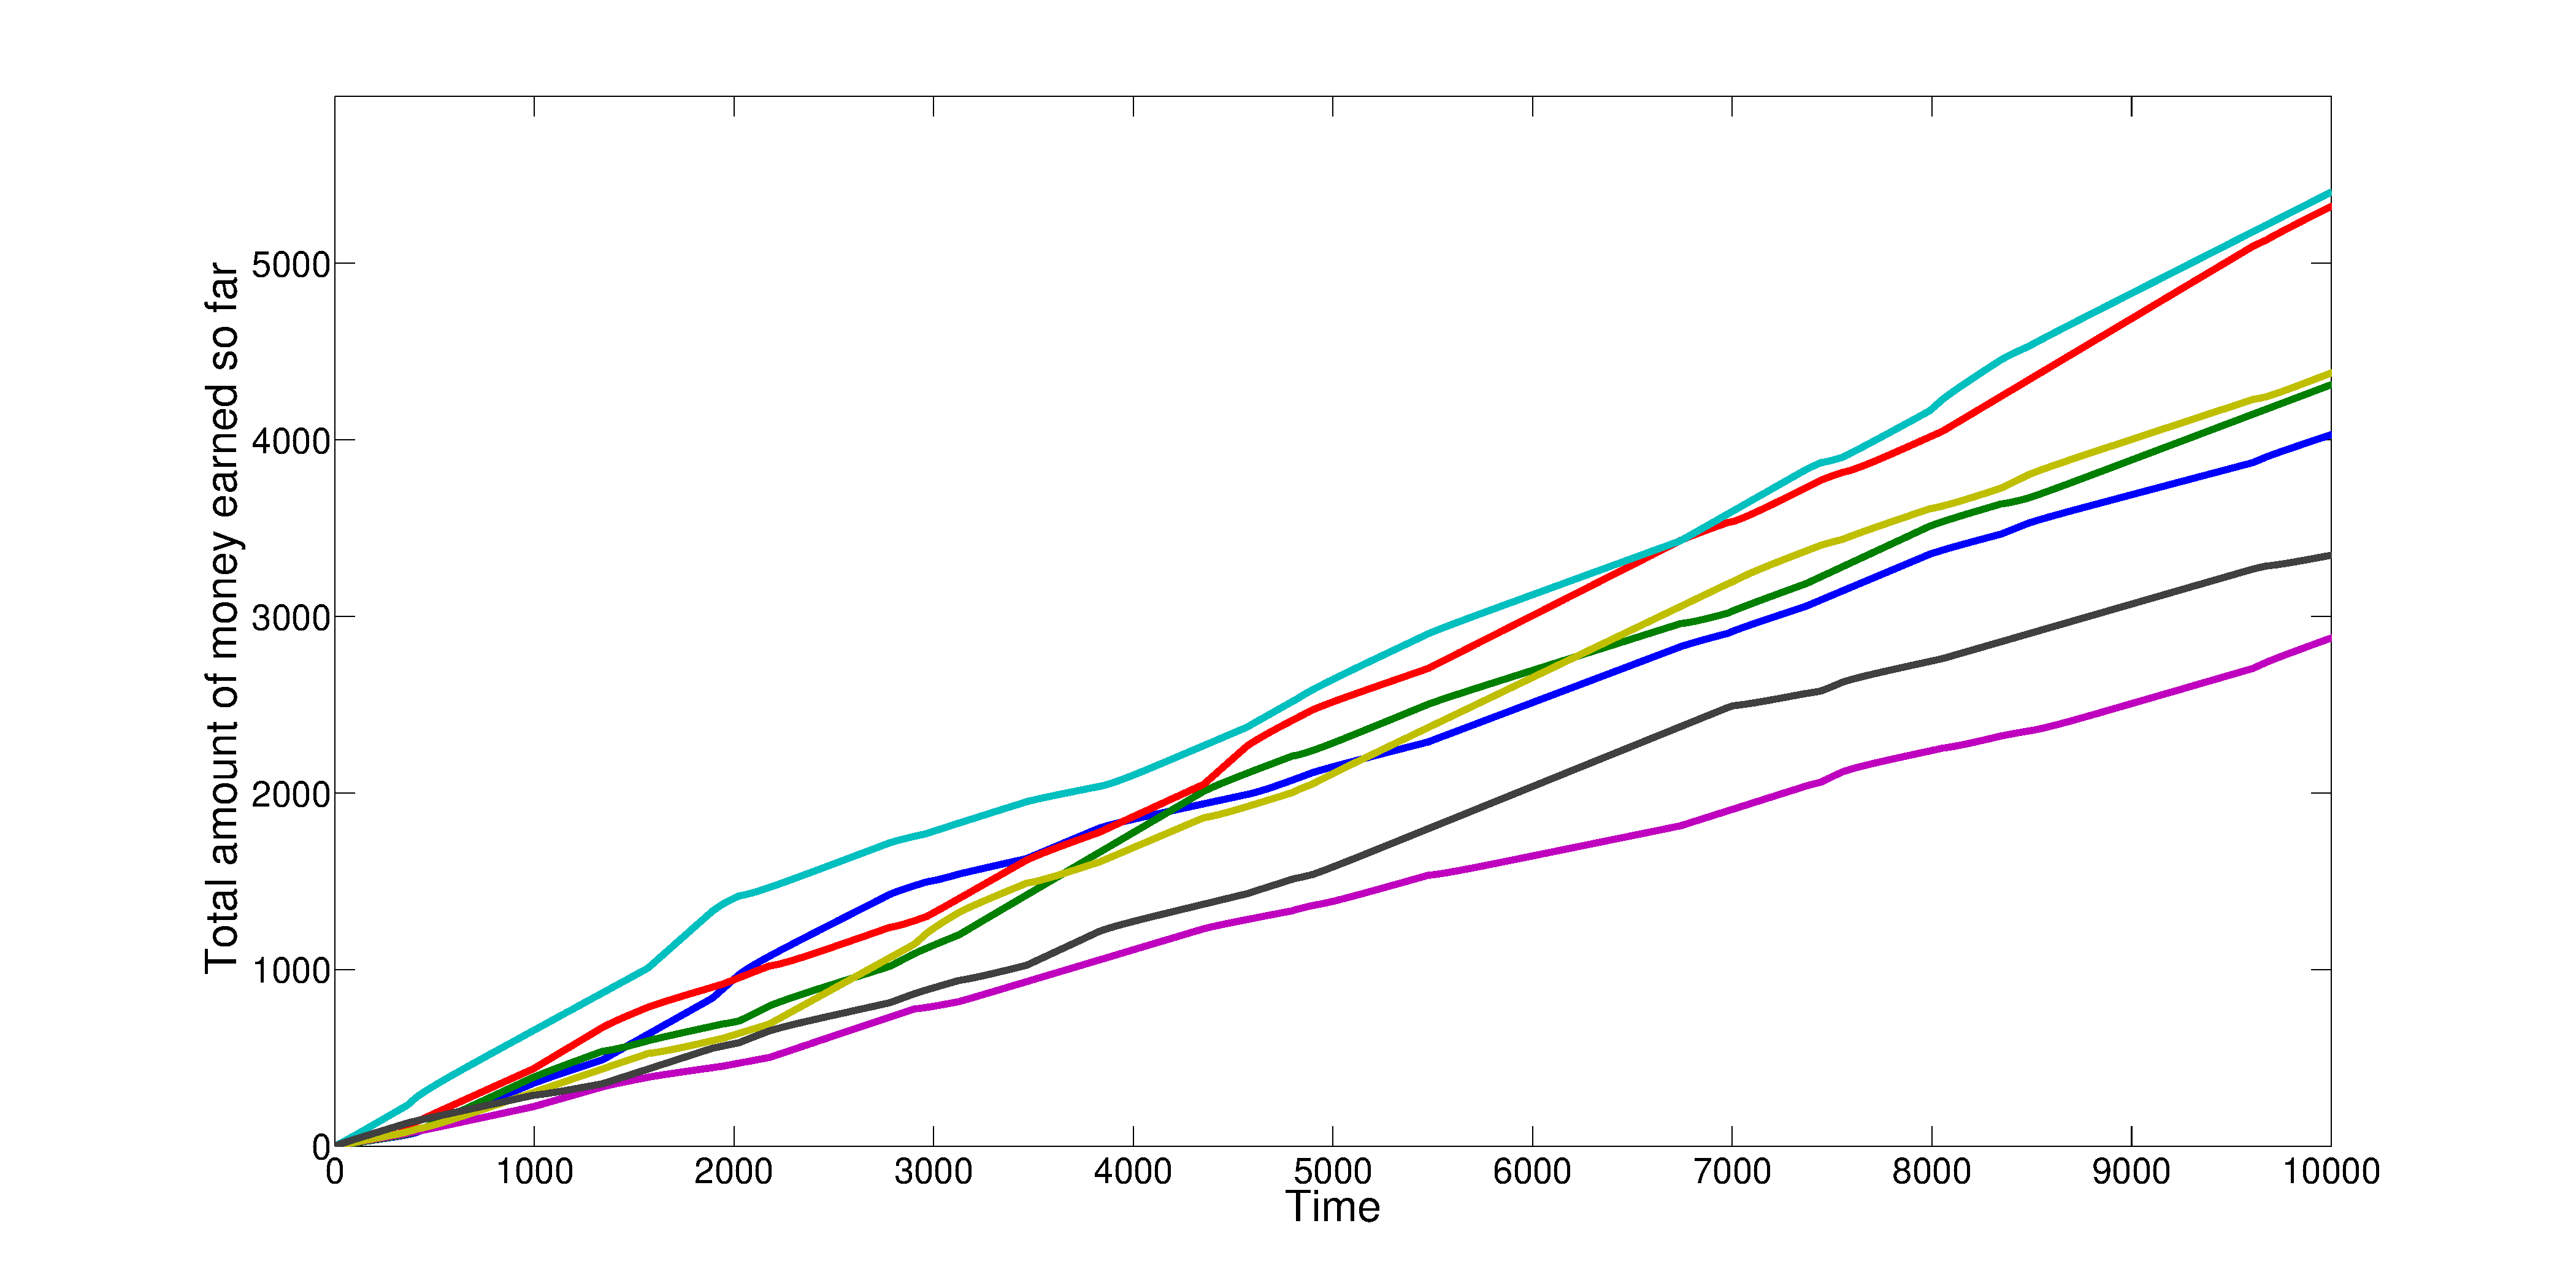
\includegraphics[width=0.9\textwidth]{../figures/totalmoney.pdf}
	\caption{Total money earned by each of the workers. It illustrates how the social inequalities are steadily increasing, and the hierarchy of the society stays the same over during the simulation.}
	\label{fig:sim1totalmoney}
\end{figure}

The randomness used in generation of the productivities $P_{ij}$ and of the abilities $A_i$ allow the inspection of social inequality. Both quantities have a similar influence, with the difference that the differences in $P_{ij}$ are both task- and worker-specific, while the differences in $A_i$ are worker-specific. Setting the standard deviation of the distributions to zero would result in a model with much less social inequality, which is not the scope of the present model. The larger the standard deviation, the more pronounced the social inequalities will be. Figures~\ref{fig:sd1} and \ref{fig:sd2} illustrate the influence of the standard deviation on social inequality.

\begin{figure}[h!]
	\centering
	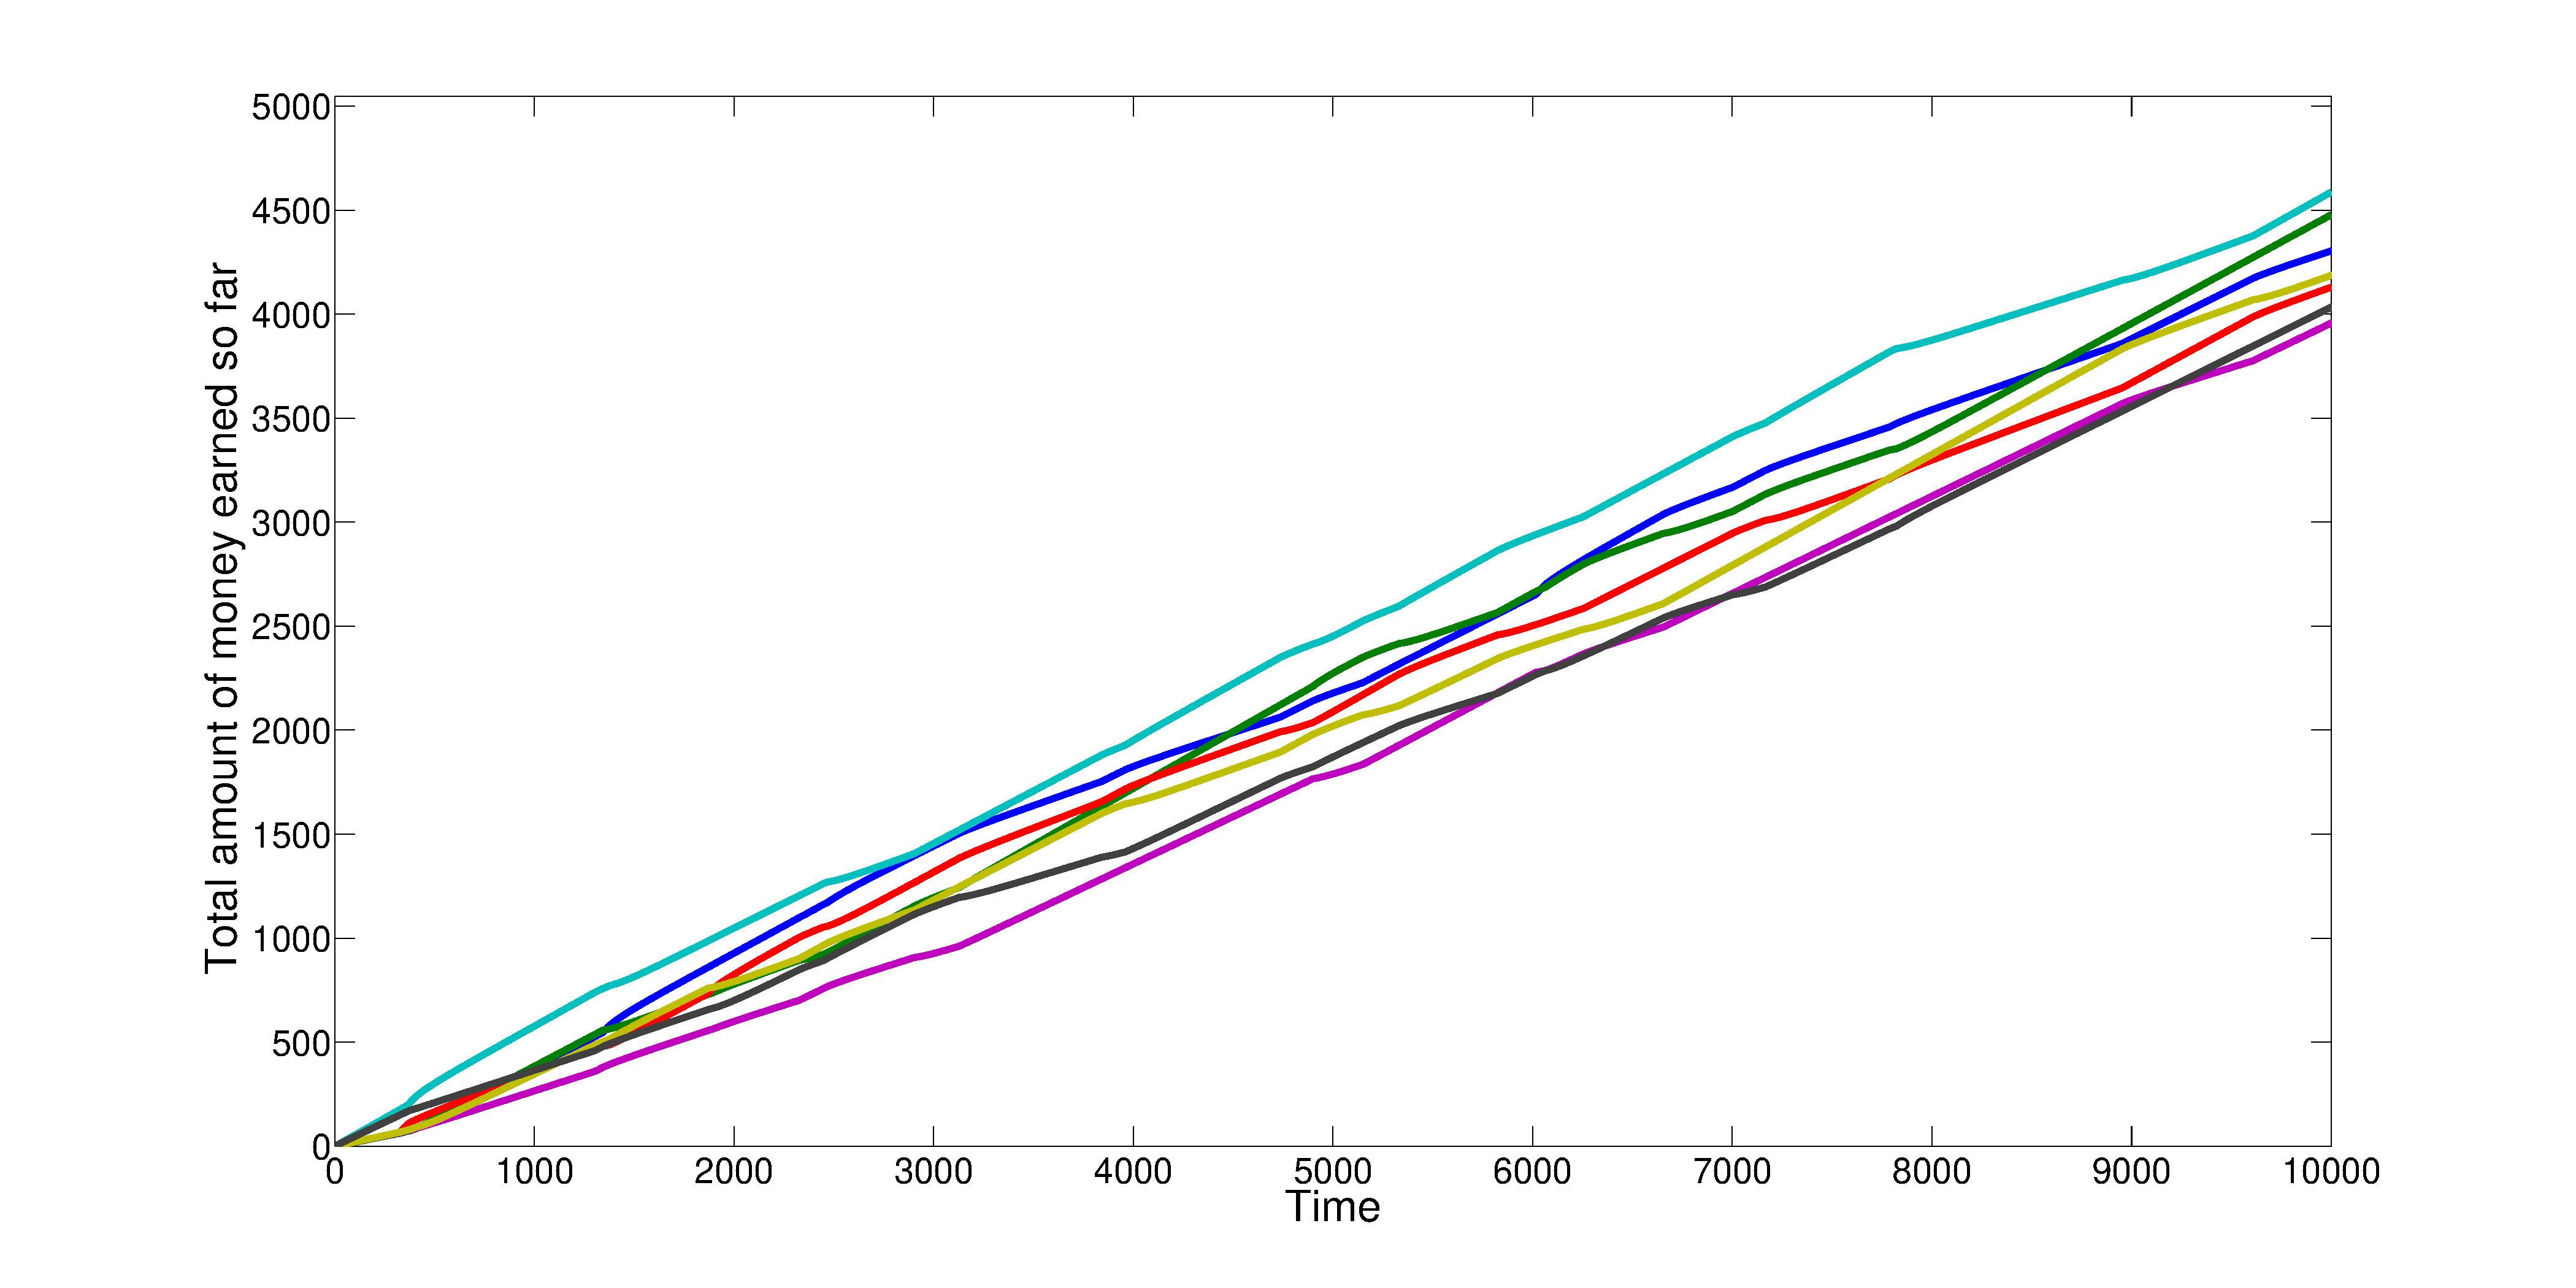
\includegraphics[width=0.9\textwidth]{../figures/sd1.pdf}
	\caption{Total money earned by each of the workers. But for $P_\sigma=0.2$ and $A_\sigma=0.2$, the same parameters as in Figure~\ref{fig:sim1totalmoney} were used. The social inequalities remain narrow and do not increase a lot with time.}
	\label{fig:sd1}
\end{figure}

\begin{figure}[h!]
	\centering
	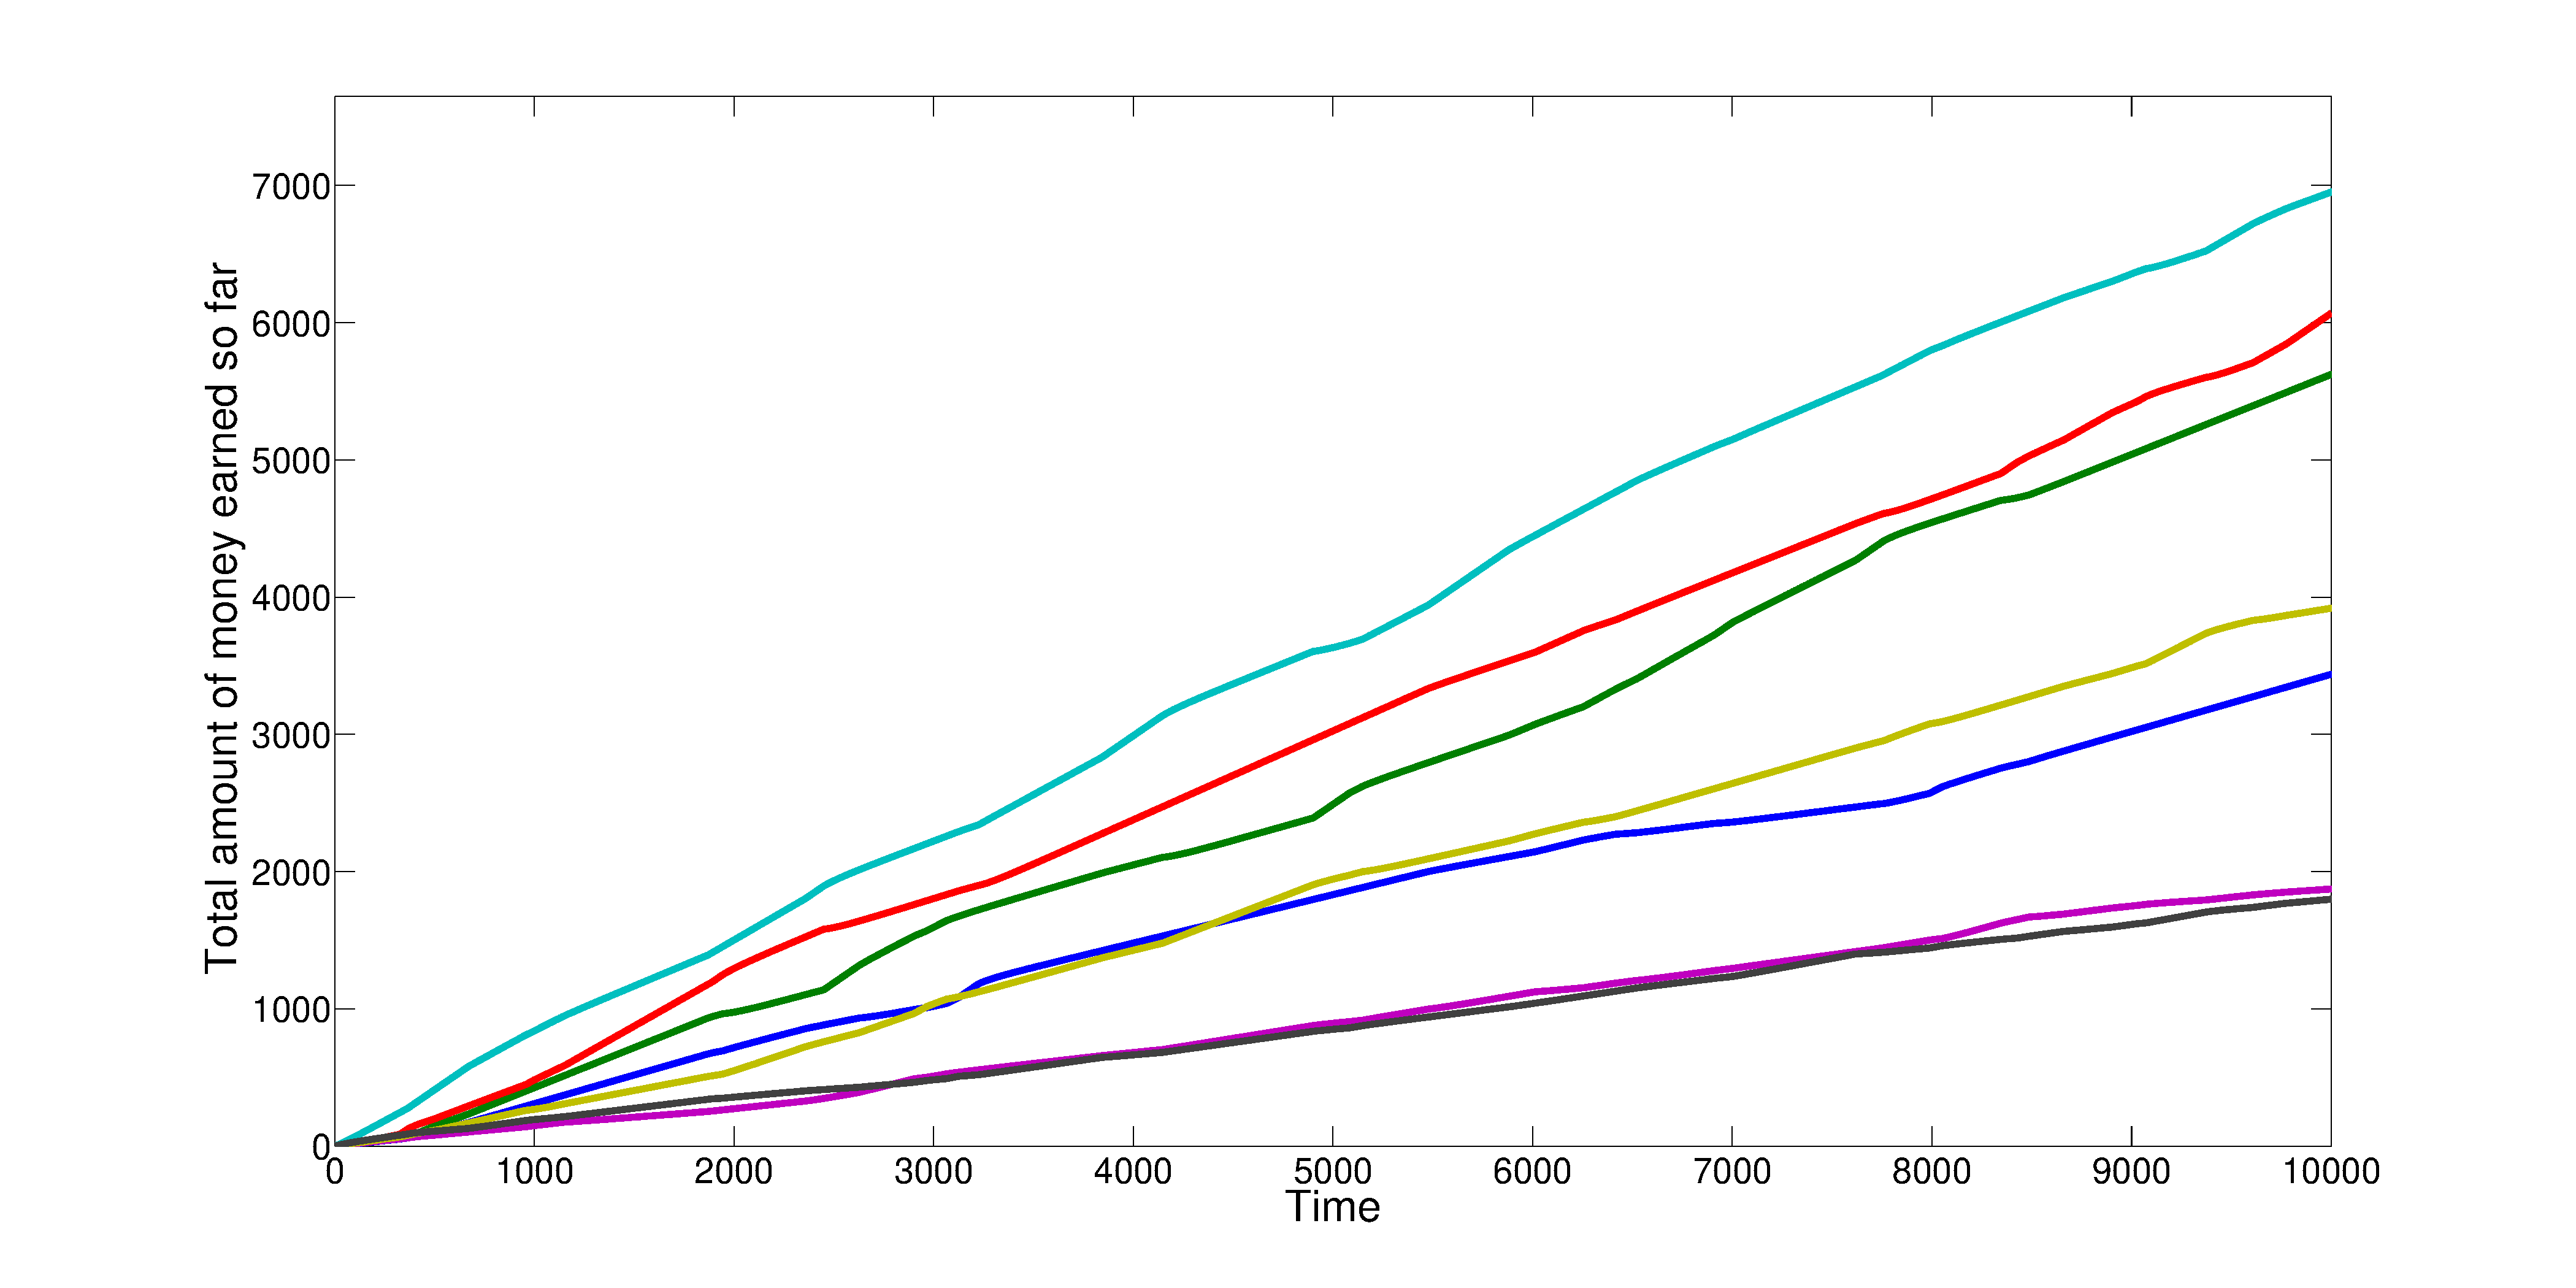
\includegraphics[width=0.9\textwidth]{../figures/sd2.pdf}
	\caption{Total money earned by each of the workers. But for $P_\sigma=1.0$ and $A_\sigma=1.4$, the same parameters as in Figure~\ref{fig:sim1totalmoney} were used. The social gap increases a lot and some workers earn several times the salary of other individui.}
	\label{fig:sd2}
\end{figure}
The boredom can be seen as the main reason for choosing a new task. Figure~\ref{fig:noboredom} was obtained by using $\zeta=0$ instead of $\zeta=0.001$ as above. It displays a prompt work specialization, illustrated by no task changes after a short equilibration period, due to the absence of boredom. 
Figure~\ref{fig:moreboredom1} and \ref{fig:moreboredom2}, on the other hand, were obtained with $\zeta=0.01$ and $B_\mu=1.5$. They show the more frequent task changes and the higher average boredom. It is to be noted that the high sensitivity to boredom in this case does not diminish the social inequalities, which can be seen in Figure~\ref{fig:moreboredom3}. The randomness in the generation of $B_{ij}^\textrm{max}$ allows the differenciated sensibility to boredom, which, as mentioned above, has an influence on the rate at which an individual will change tasks.
Another cause for a change in the task is the evolution of the market, meaning that a worker is more likely to leave his current task if a new individuum just joined the new task, thus lowering the average salary.

\begin{figure}[h!]
	\centering
	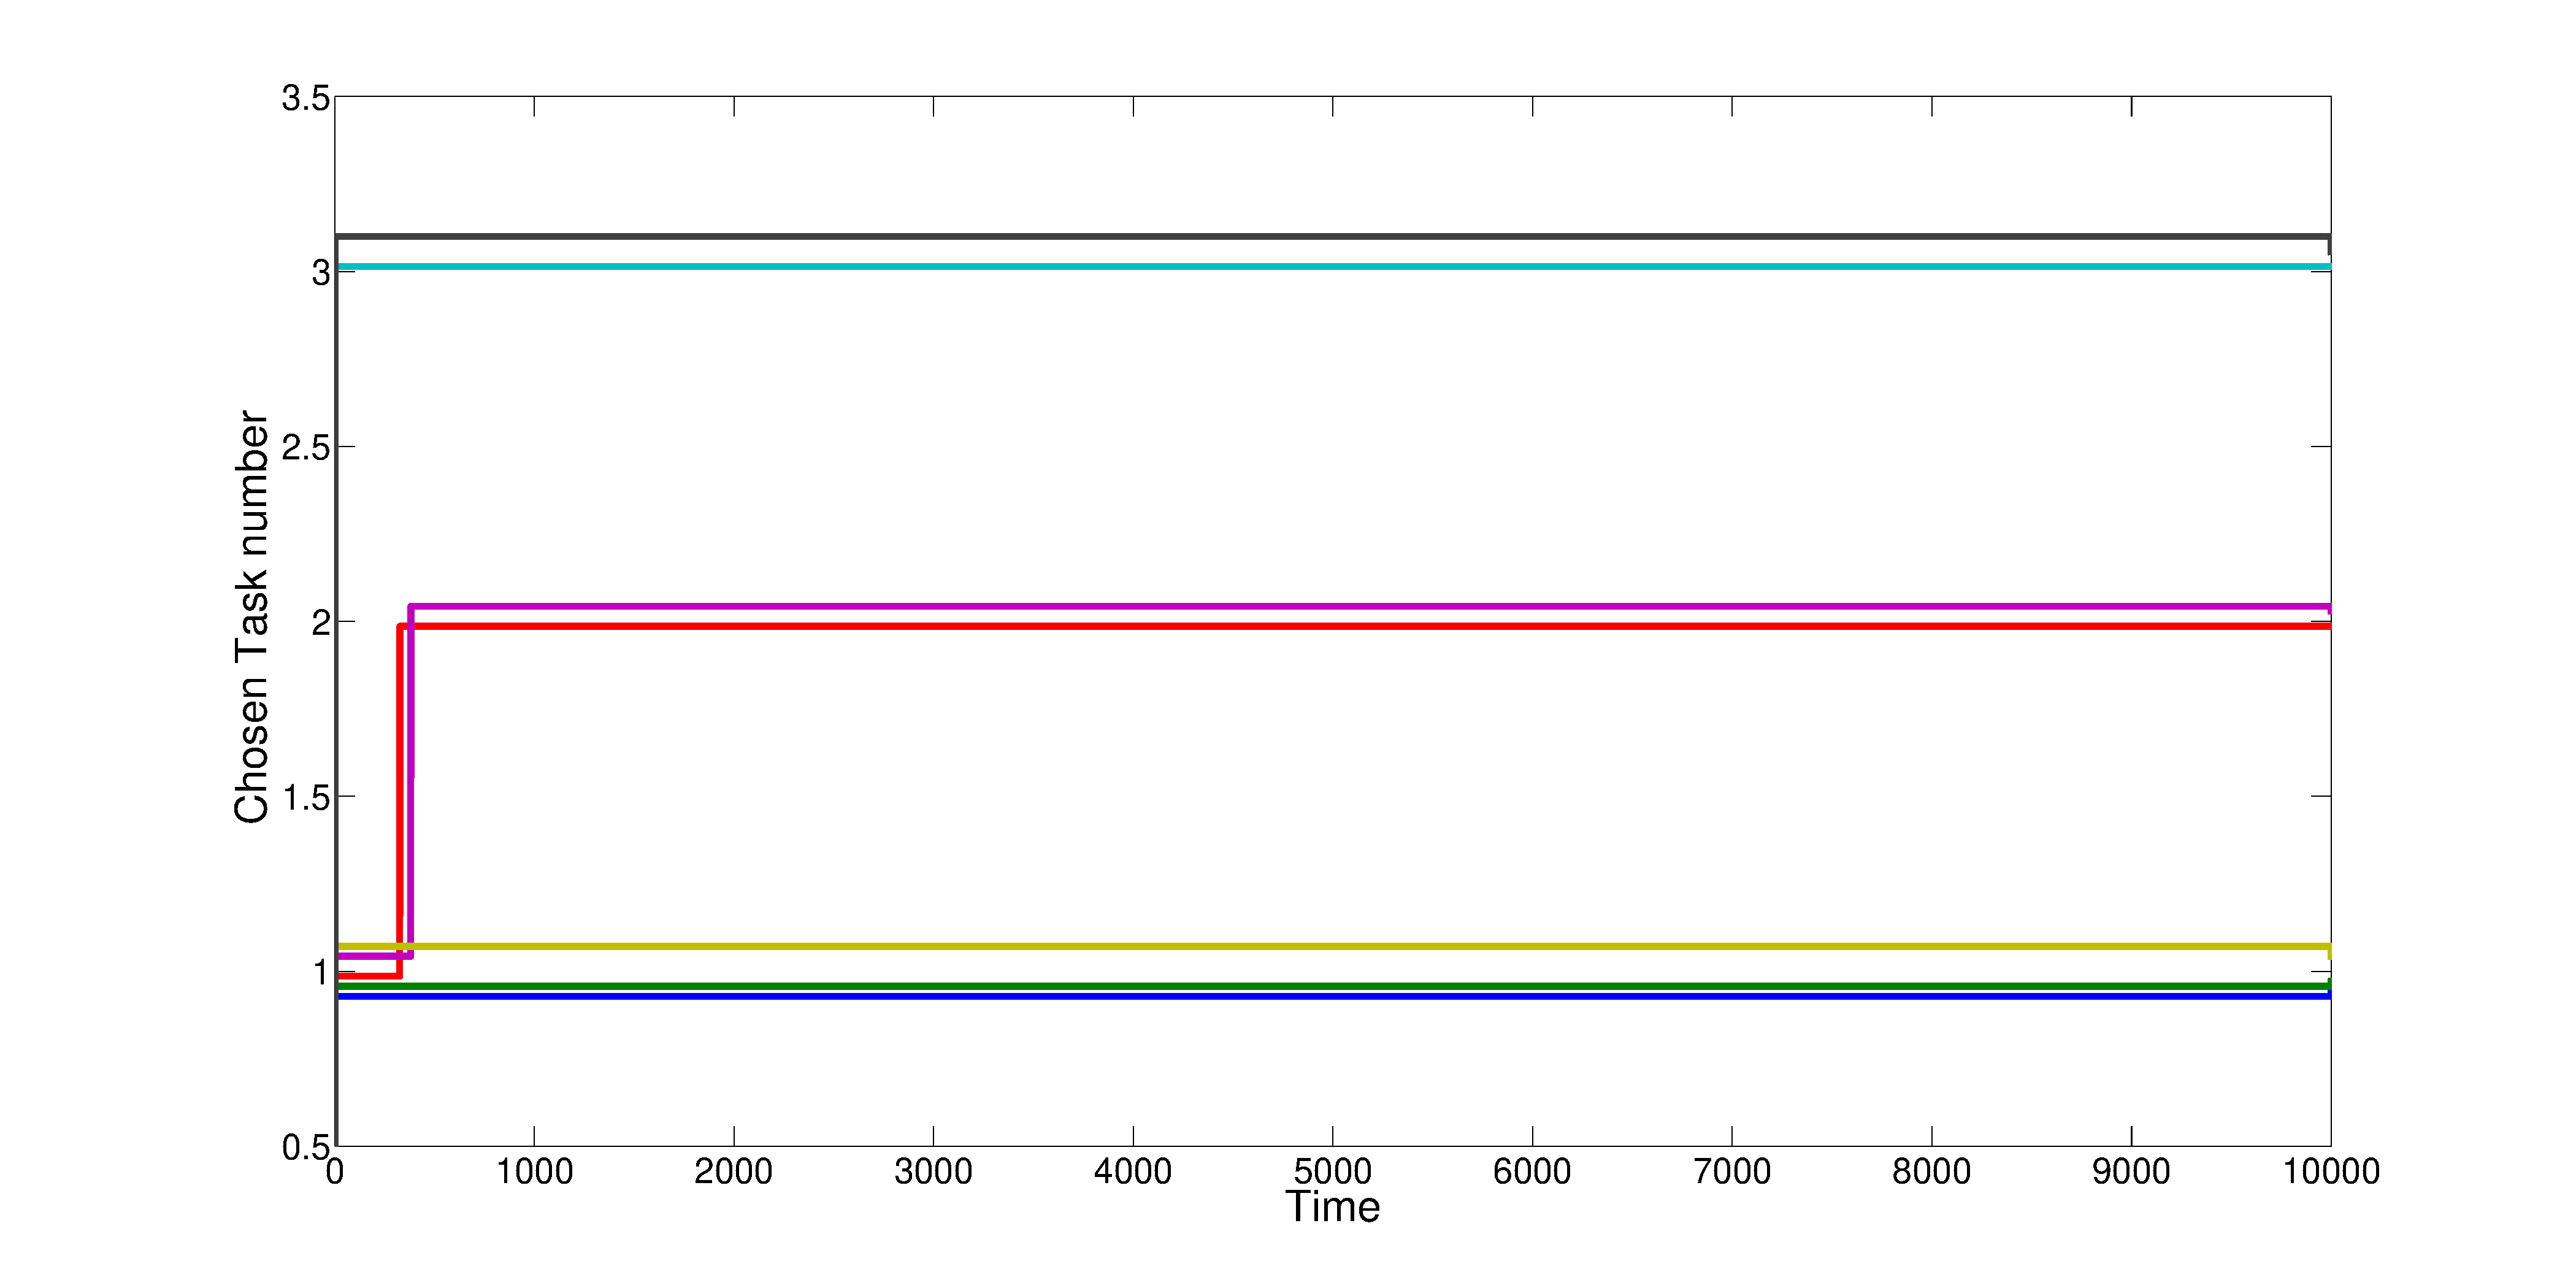
\includegraphics[width=0.9\textwidth]{../figures/noboredom.pdf}
	\caption{Chosen task number as a function of time. The same parameters as in Figure~\ref{fig:sim1task} were used but for $\zeta=0$, which imply that the workers do not experience any boredom at all. It shows an early change of task for two of the workers, after which the system does not change anymore.}
	\label{fig:noboredom}
\end{figure}

\begin{figure}[h!]
	\centering
	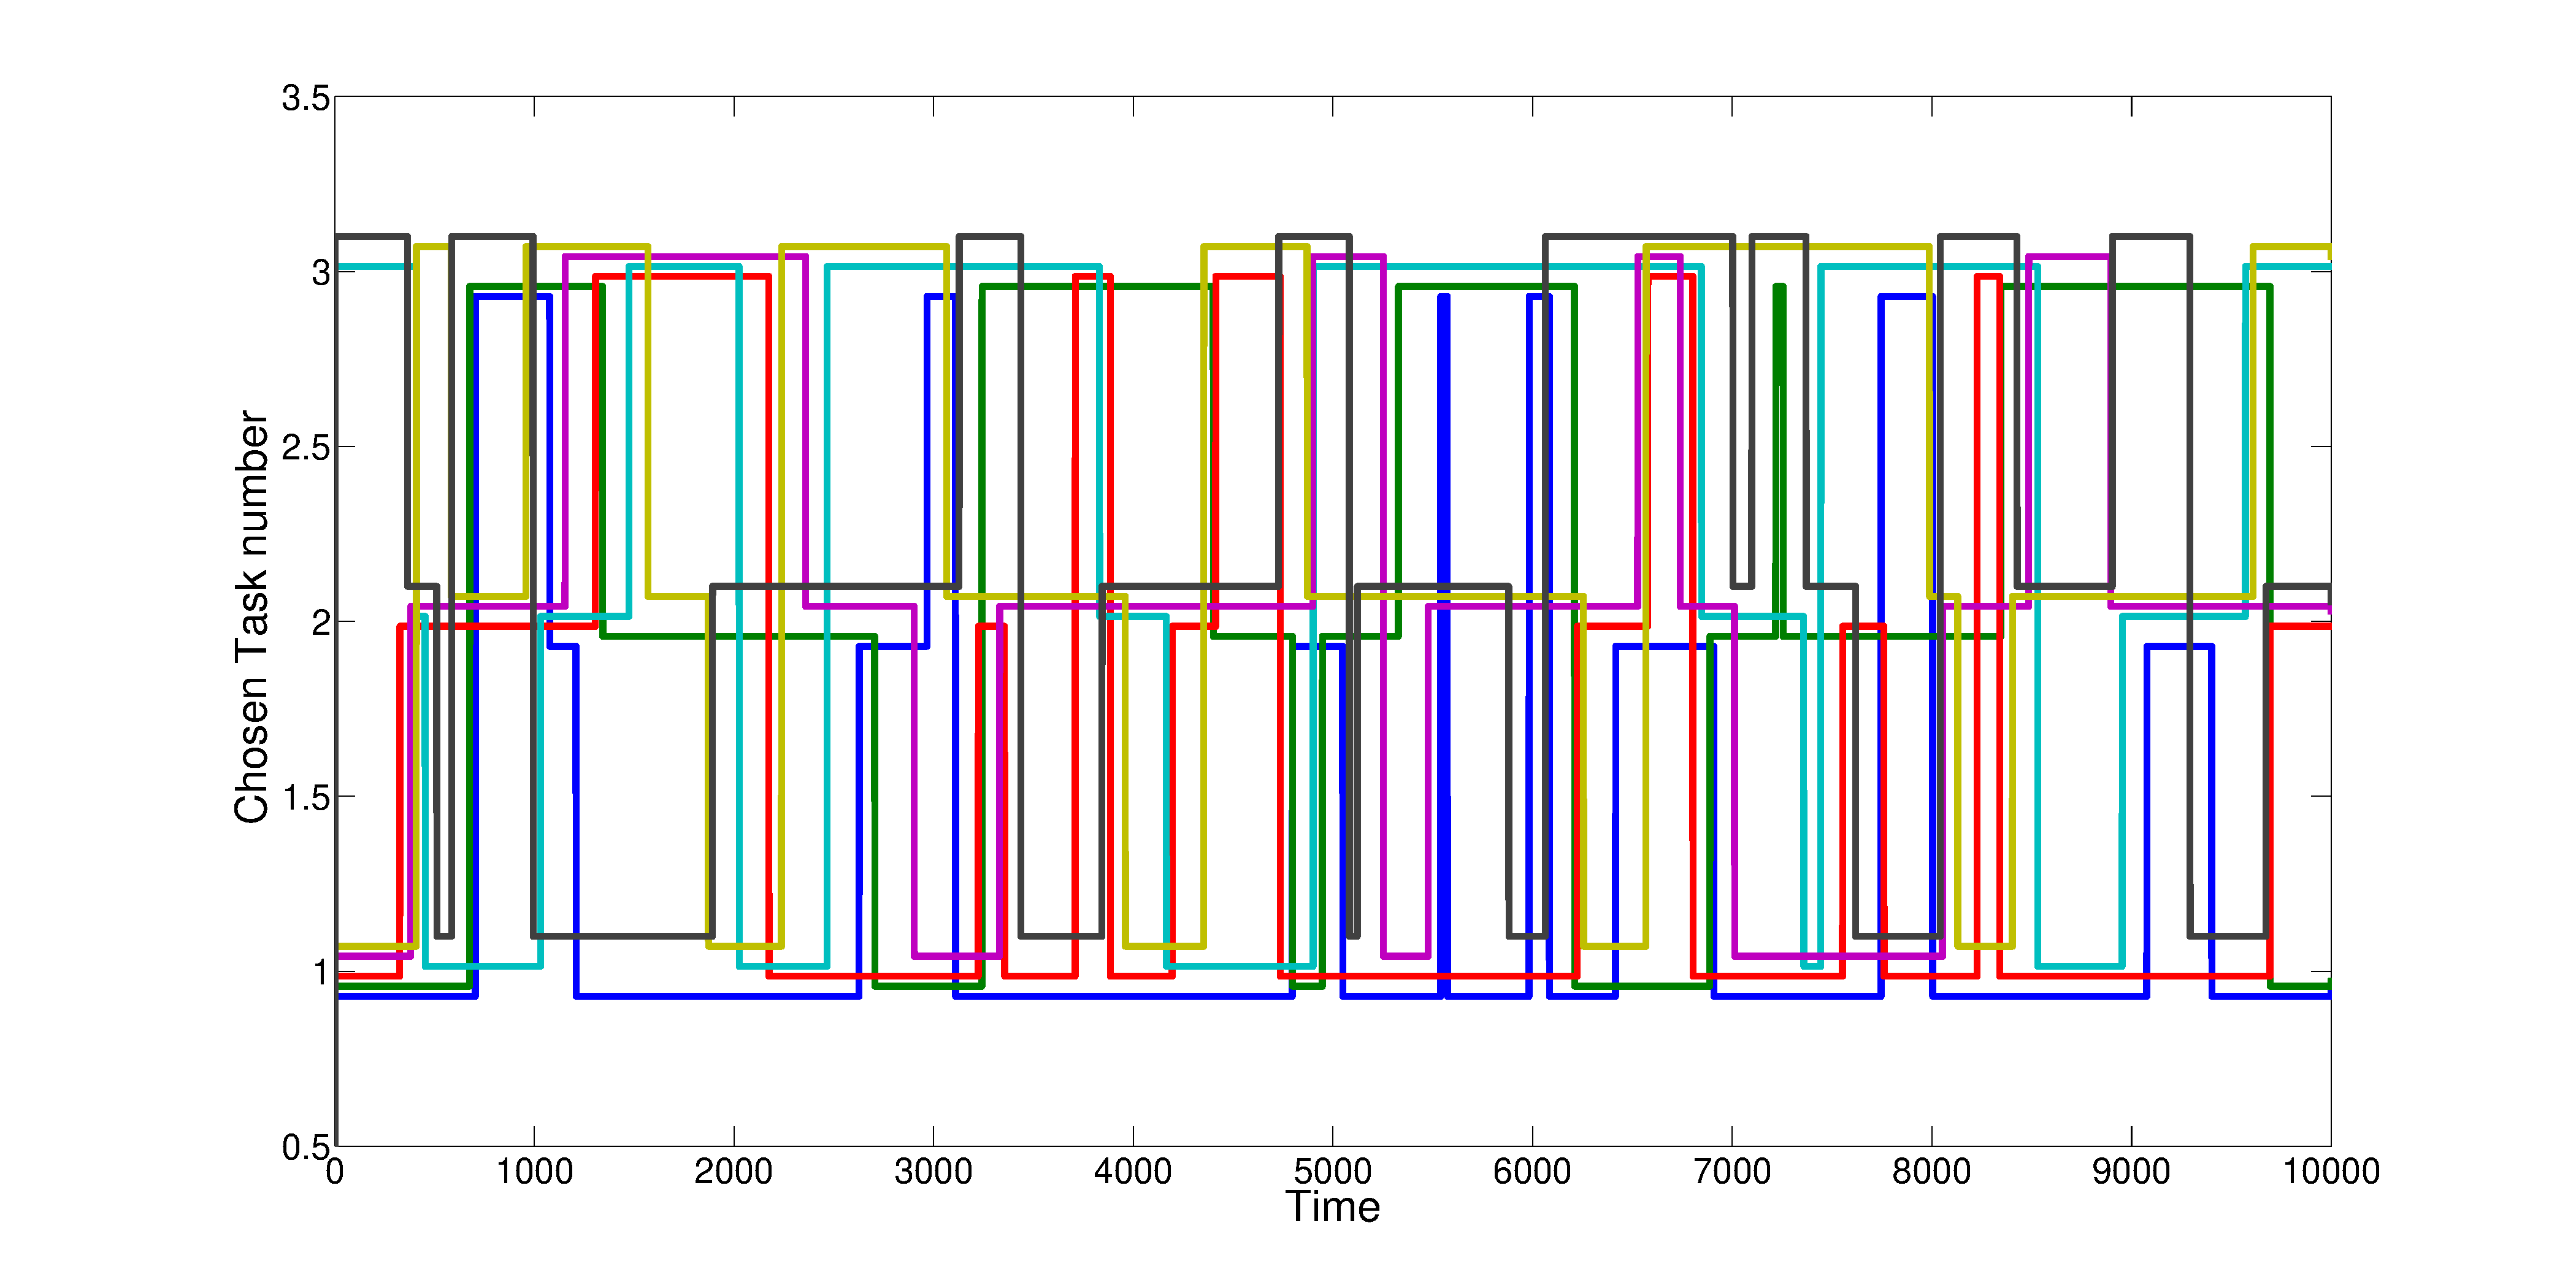
\includegraphics[width=0.9\textwidth]{../figures/moreboredom1.pdf}
	\caption{Chosen task number with $\zeta=0.01$ and $B_\mu=1.5$. All the other parameters are the same ones as used for Figure~\ref{fig:sim1task}. The very high rate of task changes is mainly due to the high average boredom, which is displayed in Figure~\ref{fig:moreboredom2}.}
	\label{fig:moreboredom1}
\end{figure}

\begin{figure}[h!]
	\centering
	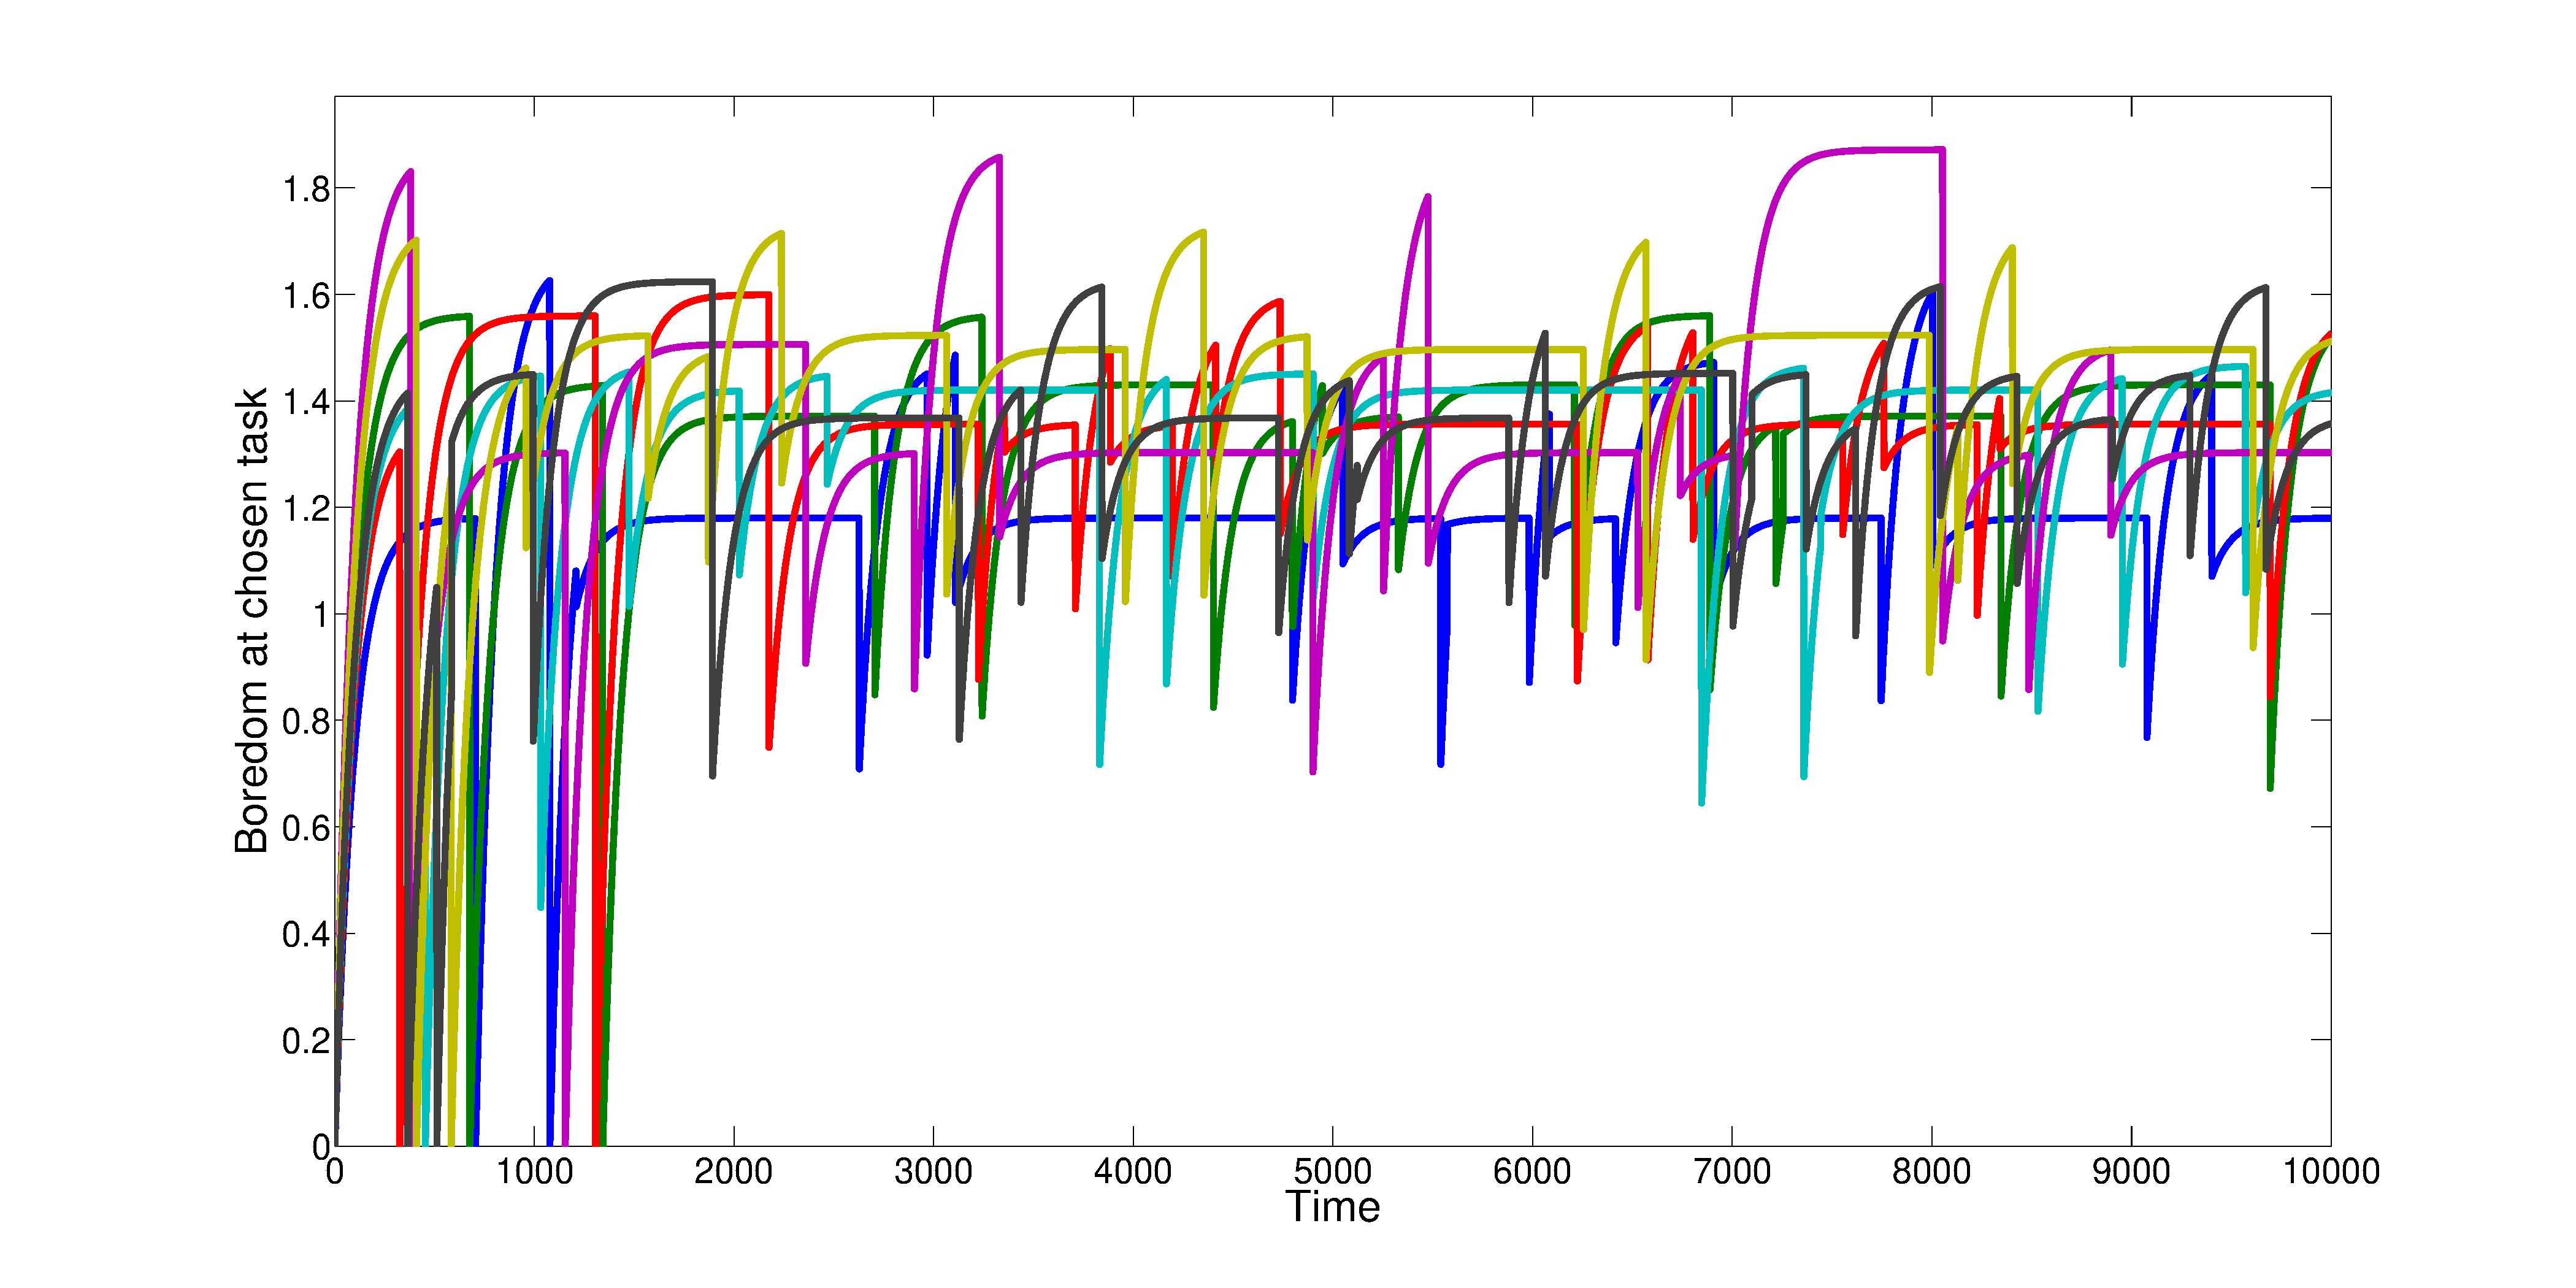
\includegraphics[width=0.9\textwidth]{../figures/moreboredom2.pdf}
	\caption{Boredom experienced by the workers at their current task for high maximal boredoms and a high fatigability.}
	\label{fig:moreboredom2}
\end{figure}

\begin{figure}[h!]
	\centering
	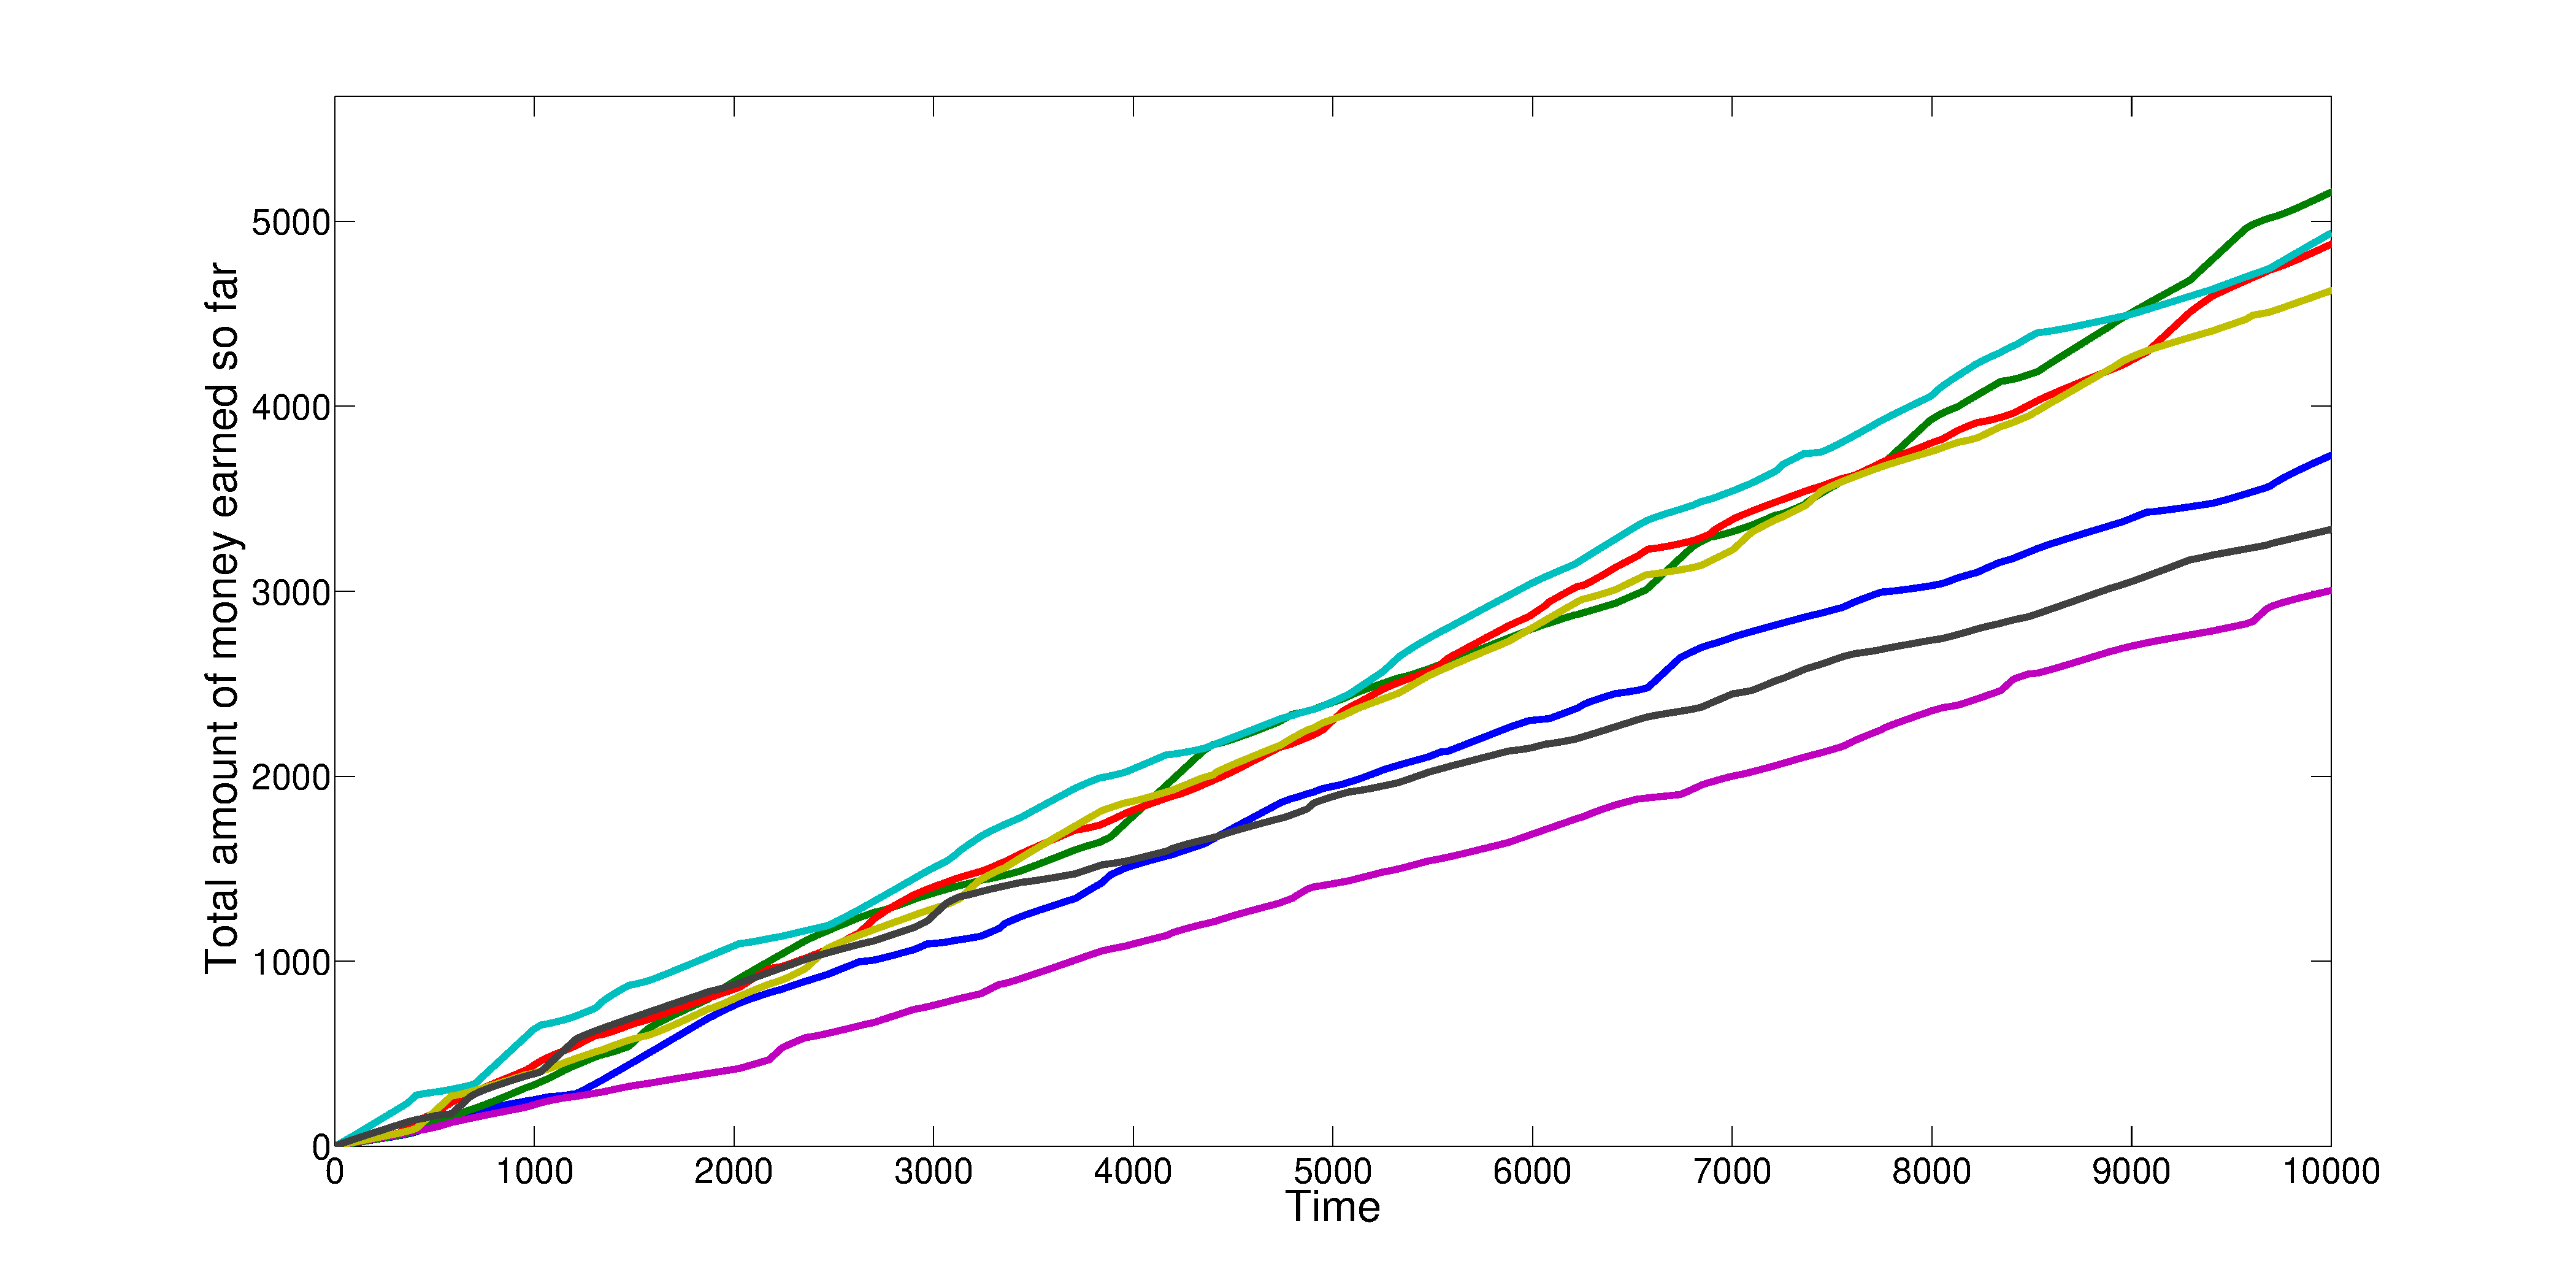
\includegraphics[width=0.9\textwidth]{../figures/moreboredom3.pdf}
	\caption{Total amount of money earned by the workers in the case where the fatigability and the maximal boredoms are high. Despite more fluctuations in comparison with Figure~\ref{fig:sim1totalmoney}, the social inequalities are still pronounced.}
	\label{fig:moreboredom3}
\end{figure}

The parameter $p_s$ becomes important when task changes become frequent and a smaller value for $p_s$ will result in less frequent task changes. However, changing $p_s$ above a specific threshold will have a negligible influence, as the additional time a worker has to wait after a new task has become more profitable will change only little.
